\documentclass[12pt,a4paper,twoside,openright,pdftex]{book}
                              % Reproservice prints on G4, which is about 80% of A4.
                              % With this scale, 12pt font becomes 9.6pt.
                              % https://www.chalmers.se/insidan/SV/arbetsredskap/kommunikation/tryck-och-layout/mallar-for-trycksaker/avhandlingens-utformning

\synctex=1                    % instead of "pdflatex -synctex=1 main"

\usepackage{lipsum}           % generating fill-in text for this thesis template

\usepackage{ifthen}           % if-then-else (to choose PhD/Lic titles)

\usepackage[utf8]{inputenc}   % unicode letters in the input tex document

\usepackage[T1]{fontenc}      % unicode letters in the output pdf

\usepackage{amssymb, amsmath} % math symbols

\usepackage{lmodern}          % better font

\usepackage{microtype}        % micro typesetting (on errors use draft to disable)

\usepackage{booktabs}         % better table formatting

\usepackage[pdftex]{graphicx} % images

\usepackage{tikz}             % simply amazing graphics library for LaTeX
\usetikzlibrary{calc}

\usepackage[%                 %
  a4paper%
  ,twoside                    %
  ,inner=2.5cm                % inner margin
  ,outer=2.5cm                % outer margin
  ,bindingoffset=1cm       % additional binding offset on the inner side
  ,bottom=3cm
]{geometry}                   % Adjust the margins

\usepackage{fancyhdr}         % fine-tuning of headers
\pagestyle{fancy}

\usepackage{emptypage}        % no page numbers in headers/footers of blank pages between chapters

\usepackage{setspace}         % for \setstretch in captions

\usepackage[%
    margin=0.75cm,            % make captions narrower than the main text
    font={small,stretch=0.80}%%
  ]{caption}                  % captions

\usepackage{subcaption}       % subcaption -- subfigures (replaces subfig)

\usepackage{url}              % handles URLs correctly (e.g. DOI, software links)

\usepackage[%
  url=true,%                  % print URLs in references, except for the ones removed below
  backend=biber,%             % use biber instead of bibtex
  style=authoryear,%          % cite as: (Author 2008)
  maxbibnames=10,%            % max names in bibliography
  maxcitenames=2,%            % max names in citation
  mincitenames=1,%            % if there are more than maxcitenames, shrink to this
  backref=true,%              % prints page numbers (wrong with \frontmatter and hypertexnames=false)
  dashed=false                % do not replace repeated author with a dash in bibliography
]{biblatex}                   % Modern bibtex replacement (bibliography mgmt)

\usepackage[%
   pdftex%
  ,hidelinks%
  ,linktoc=all%               % part of a ToC entry to be made into a link (section/page/all)
  ,unicode%
  ,bookmarksopen=true%
  ,bookmarksopenlevel=0
  ,bookmarksnumbered=true
  %,hypertexnames=false,%     % Correct ToC hyperlinks even with chapter counter reset, but broken biblatex backref.
                              % Instead of using hypertexnames=false, use \renewcommand on \theHchapter, 
                              % see http://tex.stackexchange.com/a/6099
  %,draft                     % draft can be used to avoid some strange links errors
]{hyperref}                   % links in pdf document

\usepackage{bookmark}         % Create pdf bookmarks in one go
\usepackage{nomencl}
\usepackage{float}
\makenomenclature
% This will add the units
%----------------------------------------------
\newcommand{\nomunit}[1]{%
\renewcommand{\nomentryend}{\hspace*{\fill}#1}}
%----------------------------------------------

%%% Flow chart stuff:
\usepackage{tikz}
\usetikzlibrary{shapes.geometric, arrows}
\tikzstyle{startstop} = [rectangle, rounded corners, minimum width=2cm, minimum height=1cm,text centered, draw=black, fill=red!30]
\tikzstyle{io} = [rectangle, rectangle, minimum width=0.0cm, minimum height=0.7cm, draw=none, fill=white]
\tikzstyle{process} = [rectangle, minimum width=1cm, minimum height=1cm, text centered, draw=black, fill=orange!30]
\tikzstyle{decision} = [diamond, minimum width=3cm, minimum height=0.7cm, text centered, draw=black, fill=green!30]
\tikzstyle{arrow} = [thick,->,>=stealth]
\tikzstyle{white-box} = [rectangle, minimum width=2cm, minimum height=0.7cm, text centered, draw=black, fill=white]
\tikzstyle{black-box} = [rectangle, minimum width=2cm, minimum height=0.7cm, text centered, draw=black, fill=black, text=white]

\def\equationautorefname~#1\null{Eq.#1\null}
\def\figureautorefname~#1\null{Fig.#1\null}
\def\tableautorefname~#1\null{Tab.#1\null}

\usepackage{tocloft}  % No page number of appended papers

% % % Biblatex

\addbibresource{library.bib}  % Bibliography file
\renewcommand{\cite}{\parencite}

% Remove URLs from common (easy-to-find) entries.
\AtEveryBibitem{%
  \ifboolexpr%
    {%
      test { \ifentrytype{book} }
      or
      test { \ifentrytype{inbook} }
      or
      test { \ifentrytype{inproceedings} }
      or
      test { \ifentrytype{incollection} }
      or
      test { \ifentrytype{article} }
    }
    {\clearfield{url}}
    {}%
}
% End Biblatex


% % % New environments

% \newenvironment{env-name}[optional-number-of-args]{insert-before}{insert-after}

% \newenvironment{env-name}[optional-number-of-args][default-args]{insert-before}{insert-after}

\newenvironment{abstract}{
  \begin{center}
    {\bfseries Abstract\par}  % \bfseries - some bold font, \par - end of paragraph (as empty line)
  \end{center}
  \quotation                  % extra indent from left and right
  \noindent
}
{\par\endquotation}

\newenvironment{keywords}%
{{\bfseries Keywords:}}%
{\par}%
% % % End new environments


% Begin page content adjustments for putting more text on pages.
\renewcommand{\topfraction}{.85}       % max fraction of floats at top
\renewcommand{\bottomfraction}{.7}     % max fraction of floats at bottom
\renewcommand{\textfraction}{.15}      % minimal text wrt. figs
\renewcommand{\floatpagefraction}{.66} % fraction for page of floats. floatpagefraction MUST be less than topfraction 
\renewcommand{\dbltopfraction}{.66}    % fit big float above 2-col. text
\renewcommand{\dblfloatpagefraction}{.66}
\setcounter{topnumber}{9}
\setcounter{bottomnumber}{9}
\setcounter{totalnumber}{20}
\setcounter{dbltopnumber}{9}
\widowpenalty=300                             % widow (at the beginning of page)
\clubpenalty=300                              % orphans (at the end of page)
\setlength{\parskip}{0ex plus 0.5ex}  % space between paragraphs
% End page content adjustments

% % %
% Begin remove page numbers from the "Part I" pages
\fancypagestyle{veryempty}{% no headers, no page numbers
  \fancyhf{} % remove everything
  \fancyfoot{}
  \renewcommand{\headrulewidth}{0pt} % remove lines as well
  \renewcommand{\footrulewidth}{0pt}
}
\makeatletter
\renewcommand\part{%
  \if@openright
    \cleardoublepage
  \else
    \clearpage
  \fi
  \thispagestyle{veryempty}%
  \if@twocolumn
    \onecolumn
    \@tempswatrue
  \else
    \@tempswafalse
  \fi
  \null\vfil
  \secdef\@part\@spart}
\makeatother
% End remove page numbers from the "Part I" pages


% % % % %

% Common things used both in the thesis and in the defence announcement

\newcommand\thesistype{Lic} % PhD or Lic

\newcommand\thesistitle{System Identification of Model Ship Dynamics in Calm Waters}
\newcommand\thesissubtitle{} % if empty leave only {}
\newcommand\thesisauthor{Martin Alexandersson}

\newcommand{\thesiscoverimage}{kappa/images/jeremy-bishop-QtIXL7C4bB0-unsplash.jpg} % Cover image. Comment away (not leave empty) if not needed
\newcommand{\thesiscoverdescription}{ }  % Leave {} if no description of the cover image needed

\newcommand\thesisdepartment{Department of Mechanics and Maritime Sciences}
\newcommand\thesiscity{Göteborg}
\newcommand\thesismonth{October} % e.g. January, February...
\newcommand\thesisyear{2022}
\newcommand\thesisisbn{ }  % call library to get this number for PhD, leave empty for Lic
\newcommand{\thesisissn}{%
  \ifthenelse{\equal{\thesistype}{PhD}}%
    {ISSN 0346-718X}% For PhD it is Chalmers PhD ISSN (call library to double-check)
    {ISSN 1403-266X}% For Lic it is Departmental reports ISSN (ask secretary)
}
\newcommand\thesisnumber{3471} % for PhD this is "Ny serie nr" and looks like 3452 (call library to get your number), for Lic it is departmental report number and looks like R001 (ask department secretary)

% Defence information
\newcommand\defenceday{18} % e.g. 14th
\newcommand\defencemonth{\thesismonth} % e.g. January, February...
\newcommand\defenceyear{\thesisyear} % e.g. 2009, 2010...
\newcommand\defencetime{10:00} % e.g. 10:00, 13:00...
\newcommand\defenceroom{EA} % e.g. "EA", "HC4"...
\newcommand\defenceaddress{Hörsalsvägen 11, Göteborg} % from where the \thesislocation can be accessed
\newcommand\defenceopponent{Dr. rer. nat. Carsten Sinz}
\newcommand\defenceopponentdepartment{Institute for Theoretical Computer Science}
\newcommand\defenceopponentuniversity{Karlsruhe Institute of Technology, Germany}
     % author, title, etc

\title{\thesistitle}
\author{\thesisauthor}

\pdfinfo{%
  /Title (\thesistitle)
  /Author (\thesisauthor)
}

% Compression options
\pdfminorversion=5
\pdfobjcompresslevel=3  % compression requires \pdfminorversion at least 5
\pdfcompresslevel=9     % compression requires \pdfminorversion at least 5


\begin{document}

\pagenumbering{alph}

\thispagestyle{empty}

\begin{tikzpicture}[remember picture, overlay]
  \node [anchor=north west, inner sep=0pt]  at (current page.north west)
     {\includegraphics[width=\paperwidth]{frontmatter/standard-cover-header}};

  % Cover image
%  \ifdefined\thesiscoverimage
%    \node [inner sep=0pt,anchor=north west]  at
%      ($ (current page.north west) + (1.8cm, -7cm) $)
%       {\includegraphics[width=11cm]{\thesiscoverimage}};
%  \fi

    \node [inner sep=0pt,anchor=north west]  at
      ($ (current page.north west) + (1.8cm, -7cm) $)
       {
       \begin{figure}
           
           \begin{subfigure}[b]{0.3\textwidth}
           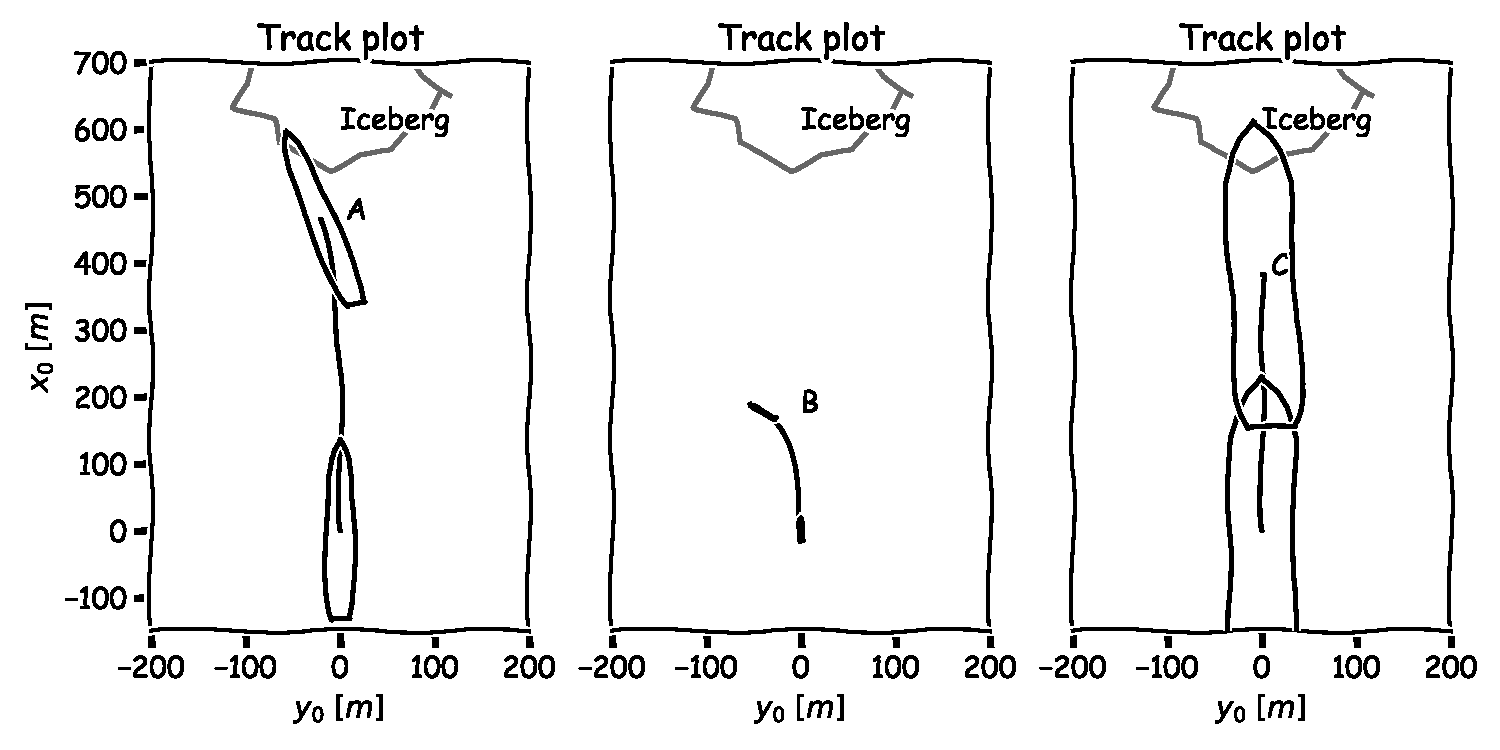
\includegraphics[width=3cm]{kappa/images/strip_1.pdf}
           \end{subfigure}
           
       \end{figure}
       
       
       };

  % Title
  \node [inner sep=0pt,anchor=south west, text width=17cm]  at
    ($ (current page.north west) + (1.8cm, -22.5cm) $)
     {
       \begin{spacing}{2}
         \textnohyphenation{\Huge \bfseries \textls*[40]{\thesistitle}}
        \end{spacing}
     };

  % Name
  \node [inner sep=0pt,anchor=north west, text width=16cm]  at
    ($ (current page.north west) + (1.8cm, -23.5cm) $)
     {\LARGE \textsc{\textls*[80]{\MakeUppercase{\thesisauthor}}}};

  % University
  \node [inner sep=0pt,anchor=north west, text width=16cm]  at
    ($ (current page.north west) + (1.8cm, -25.5cm) $)
     {
     \begin{spacing}{1.05}
     \textit{\large{Department of \thesisdepartment}}
     \par \vspace{0.15cm} \noindent
     \small \textsc{\textls*[80]{CHALMERS UNIVERSITY OF TECHNOLOGY}}
     \par \vspace{0.03cm} \noindent
     \large{Gothenburg, Sweden \thesisyear}
     \end{spacing}
   };

\end{tikzpicture}

\cleardoublepage  % advance two pages

\setcounter{page}{1}  % restart page numbering

\pagenumbering{roman}


\frontmatter                  % roman page numbers

{
\parindent 0 pt
\centering
\thispagestyle{empty}         % no page numbers here


\begin{normalsize}{\uppercase Thesis for the degree of 
\ifthenelse{\equal{\thesistype}{PhD}}{Doctor of Philosophy}{Licentiate of Engineering}}
\end{normalsize}

\vspace{3 cm}

{\large \textbf{\thesistitle} \par}
\vskip 1pc
{\large \thesissubtitle}
\vspace{1.5 cm}
\vspace{-10pt}

{\normalsize \MakeUppercase{\thesisauthor} \par}

\vspace{5 cm}


\includegraphics[width=35mm]{frontmatter/standard-images/chalmers_logo}
\vfill
\vspace{0.5 cm}

Department of \thesisdepartment \\
{\scshape CHALMERS UNIVERSITY OF TECHNOLOGY} \\
Gothenburg, Sweden \thesisyear

\newpage
}


\vspace*{50 pt}
{
  \thispagestyle{empty}         % no page numbers here

  \parindent 0 pt

  \thesistitle

  \thesissubtitle

  \textsc{\thesisauthor}

  \thesisisbn

  \vskip 1pc

  \copyright\enskip \textsc{\thesisauthor, \thesisyear.}

  \vskip 1pc

  \ifthenelse{\equal{\thesistype}{PhD}}{Doktorsavhandlingar}{Licentiatavhandlingar}
   vid Chalmers tekniska högskola

  \ifthenelse{\equal{\thesistype}{PhD}}{%
    Ny serie nr \thesisnumber%
  }{%
    Technical report No. \thesisnumber%
  }

  \thesisissn

  \vskip 1pc

  Department of \thesisdepartment

  Chalmers University of Technology

  SE--412 96 Göteborg, Sweden

  Telephone\enskip+ 46 (0) 31 -- 772 1000

  \vfill

  \thesiscoverdescription

  \vskip 2pc

  Typeset by the author using \LaTeX.

  \vskip 1pc

  Printed by Chalmers Reproservice

  Göteborg, Sweden \thesisyear
}

\clearpage


\thispagestyle{empty}         % no page numbers here
\vspace*{10 pc}
\hfill{\it to my family}
\vfill
\clearpage


% Add abstract to the ToC
\cleardoublepage              % advance the pages
\phantomsection               % put pdf anchor
\addcontentsline{toc}{chapter}{Abstract}  % add toc line with target at the last anchor
\chapter*{Abstract}
\vspace*{-1cm}                % More space for abstract text

% -- Importance, background/motivation
It is common today that operational data is recorded onboard ships within the Internet of Ships (IoS) paradigm. This enables the possibility to build ship digital twins as digital copies of the real ships. Predicting the ship's motions with ship dynamics could be an important sub-component of these ship digital twins. A model for the ship's dynamics can be identified based on observations of the ship's motions. 
The identified model will have model uncertainty due to imperfections and idealizations made in physical model formulations as well as uncertainty from errors in the measurement data, which can be very pronounced when using full scale operational data. It is easier to develop accurate models with low model uncertainty using data obtained in a controlled laboratory environment where the measurement errors are much lower, especially in calm water conditions. The prediction model should be able to describe scenarios that a ship has never encountered before, which is possible if much of the underlying physics has been identified. Grey-box modelling is a technique which combines operational data with physical principles to achieve this. 
 
The objective of this thesis is to 
% -- Objective/scope
\noindent \objective 

% -- Method, developed method, setting
A model development procedure is proposed to handle the model uncertainty through the selection of candidate models based on a hold-out evaluation procedure. The measurement noise is handled by an iterative preprocessor, which uses an extended Kalman filter (EKF) and a Rauch Tung Striebel (RTS) smoother that uses an initially estimated predictor model from semi-empirical formulas.

% -- Results example
It is demonstrated that the ship's roll motion with high accuracy can be described using a quadratic damping model. For the more complex manoeuvring models, multicollinearity is a large problem where the appropriate complexity needs to be selected with the bias-variance trade-off between underfitting or overfitting the data. 
Hold-out turning circle tests were predicted with high accuracy for the wPCC and KVLCC2 test case ships with models from the proposed development procedure and parameter estimation method.

% -- Conclusion 
The proposed methods can produce prediction models with high generalization given that a suitable model structure has been selected from the candidate models and an appropriate split in the hold-out evaluation of the model development process has been applied. 

\vspace{0.3cm}
\noindent\textbf{Keywords:} Extended Kalman filter, Inverse dynamics, Multicollinearity, RTS smoother, Ship digital twin, Ship manoeuvring, System identification
\cleardoublepage


\cleardoublepage              % advance the pages
\phantomsection               % put pdf anchor
\addcontentsline{toc}{chapter}{Acknowledgments}  % add toc line with target at the last anchor
\chapter*{Acknowledgments}
This thesis presents research performed since February 2020 at the Division of Marine Technology, Department of Mechanics and Marine Sciences at Chalmers University of Technology and SSPA Sweden AB (\href{www.sspa.se}{www.sspa.se}). Financial support for this research was provided by the DEMOPS project (Development of Methods for Operational Performance of Ships) funded by Swedish Transport Administration (project: FP4 2020) and D2E2F project (Data Driven Energy Efficiency of Ships) funded by Swedish Energy Agency (project: 49301-1).

I had unsuccessfully been applying for funding for PhD studies for a couple of years when Professor Wengang Mao contacting me three years ago with the offer to become a PhD student. I will always be very grateful for this offer and I'm sure that I would otherwise be still searching for funding or given up by now. Wengang has also been my main supervisor during my studies and a guide to the academic research and a tutor in statistical and machine learning methods.  

This gratitude also goes to my examiner and co-supervisor, Professor Jonas W Ringsberg,
head of the Division of Marine Technology. I have enjoyed our discussions about research methodology and how to organize a paper in academic writing, where his detailed proof reading has also been a great asset.

I also want to thank SSPA Sweden AB for allowing me to be an industrial PhD student within my current employment. Special thanks to Dr. Christian Finnsgård head of the Research Department at SSPA, for his support and good advice throughout the project. I also want to mention all personnel at SSPA who have been involved in creating the model test results, building the ship models, and conducting the experiments.

\vskip 2pc

\noindent \thesisauthor

\noindent \thesiscity, October\  2022  % Since dedication is written a month or more before the actual thesis date, \thesismonth and \thesisyear is not used here.


\cleardoublepage              % advance the pages
\phantomsection               % put pdf anchor
\addcontentsline{toc}{chapter}{List of Publications}  % add toc line with target at the last anchor
\chapter*{List of Publications}
% This page is hand-made. I could not make Biblatex to output the papers the way I wanted.

%\begin{refsection}

This thesis is based on the following appended papers:

\begin{description}
% Biblatex \fullcite{Voronov2011} would work, but it uses maxcitenames, not maxbibnames, and there is no obvious way to change maxbibnames locally and change it back afterwards.
\item[Paper~\ref{pap:rolldamping}.]
\fullcite{alexandersson_analysis_2021}

%\item[Paper~\ref{pap:motions}.] 
%\fullcite{alexandersson_prediction_2021}

\item[Paper~\ref{pap:daiyong}.] 
\fullcite{alexandersson_comparison_2022}

\item[Paper~\ref{pap:pit}.] 
\fullcite{alexandersson_system_nodate}
\\
To be submitted to Ocean Engineering

\end{description}

\vspace{1cm}

\noindent Other relevant publications co-authored by Martin Alexandersson:
\begin{description}
\normalsize
\newcommand{\ME}{{\bfseries Martin Alexandersson}}

\item
Alexandersson, M., 2009. A STUDY OF METHODS TO PREDICT ADDED RESISTANCE IN WAVES. https://doi.org/10.13140/RG.2.2.18796.69767

\item
Alexandersson, M., Korkmaz, K., Mazza, G., 2017. Virtual Captive Tests with a destroyer hull form.

\item
Alexandersson, M., Kjellberg, M., Mao, W., Ringsberg, J., 2021. Prediction of roll motion using fully nonlinear potential flow and Ikeda’s method.


\end{description}

%\end{refsection}

%\mbox{}
\makenomenclature
\nomenclature{$\displaystyle OG$}{vertical distance into water from still water to centre of gravity\nomunit{m}}
\nomenclature{$\displaystyle A_{0}$}{mid ship area coefficient}
\nomenclature{$\displaystyle BK_{B}$}{bilge keel height\nomunit{m}}
\nomenclature{$\displaystyle BK_{L}$}{bilge keel length\nomunit{m}}
\nomenclature{$\displaystyle \phi_{a}$}{initial roll amplitude\nomunit{rad}}
\nomenclature{$\displaystyle A_{44}$}{total mass moment of inertia\nomunit{kg\cdot m^2}}
\nomenclature{$\displaystyle B_{1}$}{linear damping coefficient\nomunit{Nm/(rad/s)}}
\nomenclature{$\displaystyle B_{2}$}{quadratic damping coefficient\nomunit{Nm/(rad/s^2}}
\nomenclature{$\displaystyle B_{3}$}{cubic damping coefficient\nomunit{Nm/(rad/s)^3}}
\nomenclature{$\displaystyle B_{E}$}{eddy roll damping\nomunit{Nm/(rad/s)}}
\nomenclature{$\displaystyle B_{F}$}{friction roll damping\nomunit{Nm/(rad/s)}}
\nomenclature{$\displaystyle B_{L}$}{hull lift roll damping\nomunit{Nm/(rad/s)}}
\nomenclature{$\displaystyle B_{W}$}{wave roll damping\nomunit{Nm/(rad/s)}}
\nomenclature{$\displaystyle B_{BK}$}{bilge keel roll damping\nomunit{Nm/(rad/s)}}
\nomenclature{$\displaystyle C_{1}$}{linear stiffness coefficient\nomunit{Nm/rad}}
\nomenclature{$\displaystyle C_{3}$}{stiffness coefficient\nomunit{Nm/rad^3}}
\nomenclature{$\displaystyle C_{5}$}{stiffness coefficient\nomunit{Nm/rad^5}}
\nomenclature{$\displaystyle L$}{ship perpendicular length\nomunit{m}}
\nomenclature{$\displaystyle T$}{mean draught\nomunit{m}}
\nomenclature{$\displaystyle V$}{ship speed\nomunit{m/s}}
\nomenclature{$\displaystyle beam$}{ship beam\nomunit{m}}
\nomenclature{$\displaystyle \omega_{0}$}{natural angular velocity\nomunit{rad/s}}
\nomenclature{$\displaystyle t$}{time\nomunit{s}}
\nomenclature{$\displaystyle m$}{ship mass\nomunit{kg}}
\nomenclature{$\displaystyle \bigtriangledown$}{ship displacement\nomunit{m^3}}
\nomenclature{$\displaystyle \phi$}{ship roll angle\nomunit{rad}}
\nomenclature{$\displaystyle x_0$}{ship global position\nomunit{m}}
\nomenclature{$\displaystyle x_G$}{ship longitudinal centre of gravity\nomunit{m}}
\nomenclature{$\displaystyle GM$}{ship metacentric height \nomunit{m}}
\nomenclature{$\displaystyle g$}{gravity \nomunit{kg\cdot m/s^2}}
\nomenclature{$\displaystyle y_o$}{ship global position\nomunit{m}}
\nomenclature{$\displaystyle \Psi$}{ship heading \nomunit{rad}}
\nomenclature{$\displaystyle \beta$}{ship drift angle \nomunit{rad}}
\nomenclature{$\displaystyle \rho$}{water density \nomunit{kg/m^3}}
\nomenclature{$\displaystyle D$}{propeller diameter \nomunit{m}}
\nomenclature{$\displaystyle n$}{propeller speed \nomunit{rad/s}}
\nomenclature{$\displaystyle J$}{propeller advance ratio}
\nomenclature{$\displaystyle w_p$}{propeller wake fraction}
\nomenclature{$\displaystyle w_{p0}$}{taylor wake fraction}
\nomenclature{$\displaystyle x_p$}{propeller longitudinal position \nomunit{m}}
\nomenclature{$\displaystyle X$}{ship force in longitudinal direction \nomunit{N}}
\nomenclature{$\displaystyle Y$}{ship force in transverse direction \nomunit{N}}
\nomenclature{$\displaystyle N$}{ship yawing moment \nomunit{Nm}}
\nomenclature{$\displaystyle u$}{surge velocity\nomunit{m/s}}
\nomenclature{$\displaystyle v$}{sway velocity\nomunit{m/s}}
\nomenclature{$\displaystyle r$}{yaw rate\nomunit{rad/s}}
\nomenclature{$\displaystyle I_z$}{ship yaw moment of inertia\nomunit{kg\cdot m^2}}
\nomenclature{$\displaystyle \textbf{w}$}{process noise}
\nomenclature{$\displaystyle \textbf{c}$}{control signal}
\nomenclature{$\displaystyle \delta$}{rudder angle \nomunit{rad}}
\nomenclature{$\displaystyle \delta$}{rudder angle \nomunit{rad}}
\printnomenclature

\cleardoublepage              % advance the pages
\phantomsection               % put pdf anchor
\addcontentsline{toc}{chapter}{List of Acronyms}  % add toc line with target at the last anchor
\chapter*{List of Acronyms}
% To find all three-letter acronyms in file kappa/body.tex that are outside of comments: 
% grep -o "[^%]*" kappa/body.tex | grep -o "\b[A-Z][A-Z][A-Z]\b" | sort | uniq

\begin{tabular}{ l c l }
CFD & -- & Computational Fluid Dynamics\\
DOF & -- & Degree Of Freedom\\
FFT & -- & Fast Fourier Transform\\
ODE & -- & Ordinary Differential Equation\\
OLS & -- & Ordinary Least Squares\\
PIT & -- & Parameter Identification Technique\\
SI  & -- & Simplified Ikeda\\
VMM & -- & Vessel Manoeuvring Model\\

\end{tabular}


% add Contents to PDF bookmarks, but do not add it to the 'printed' Contents
\cleardoublepage
\phantomsection
% \pdfbookmark[level]{text-to-display-in-outline}{unique-pdf-anchor-name}, chapter is level 0
\pdfbookmark[0]{Contents}{Contents}
\tableofcontents

\mainmatter                   % normal arabic page numbers

\part{Introductory chapters}

% Headers, footers
\fancyfoot{}                  % clean all
\fancyhead[RE]{\textit{\nouppercase{\rightmark}}}
\fancyhead[RO]{\thepage}
\fancyhead[LE]{\thepage}
\fancyhead[LO]{\textit{\nouppercase{\leftmark}}}

%  \begin{refsection}

%!TEX root = ../main.tex
%%%%%%%%%%%%%%%%%%%%%%%%%%%%%%%
%%%%%%%%%%%%%%%%%%%%%%%%%%%%%%%
\chapter{Introduction}
%%%%%%%%%%%%%%%%%%%%%%%%%%%%%%%
The use of twin models is a not a new idea. NASA build twin rockets for the Apollo missions, where one rocket went to the Moon and the other twin rocket stayed on Earth, as a reference object if something went wrong during the mission.  
The twin model has a lot of other usefully applications, not just for catastrophic scenarios with a failing space ship, but also for more ordinary scenarios with conventional ships. Building a real twin ship as a reference object is not realistic however, but with data recorded onboard ships it is instead possible to build a Ship Digital Twin (SDT), to serve the same purpose.
Methods for System identification of Ship Rigid Body Dynamics are presented in this thesis, to be used as sub-component in the SDTs. 

The background of modelling the SDTs with white-, black- or grey-box models is first introduced in this chapter followed by a brief literature review. The motivation and objective of this research is then stated followed by assumptions and limitations. The chapter ends with an outline of the whole thesis.

\section{Background}
Shipbuilding 4.0, at the principles of the Industry 4.0, will transform the design, manufacturing, operation, shipping, services, production systems, maintenance and value chains in all aspects of the shipbuilding 
industry \cite{stanic_toward_2018}.
The emergence of Internet-of-Things (IoT) has led to the introduction of the Internet-of-Ships (IoS) paradigm. \begin{quote} IoS is the interconnecting of sensing objects, such as ships, crews, cargoes, onboard equipments, waterway environment, waterway facilities, shore-based facilities, and other navigation elements, which are embedded with a variety of sensor and heterogeneous network technologies to enable these objects to collect and exchange data \cite{liu_internet_2016-1}.\end{quote}
Safety enhancements, route planning and optimization, energy efficiency, automatic berthing and autonomous shipping are some of the emerging applications for IoS \cite{aslam_internet_2020}.
A SDT as a digital copy of a real ship, is one approach to achieve this \cite{chen_review_2021}. 
SDTs are data-driven in contrast to the related term Virtual Prototyping (VP), which is instead model based \cite{major_framework_2021}. A SDT is generally a model for an existing ship from where data can be collected and the VPs are generally prototypes for future ships, where no operational data is yet available.

Ship dynamics is a branch of ship hydrodynamics which concerns the ship forces and motions when the ship is allowed to move and rotate in all directions. Seakeeping and Manoeuvring are the two major sub fields, where Seakeeping studies the  behaviour of a ship in a seaway, under the influence of the external waves, currents and winds. Calm water conditions, lacking the external waves, are further assumed in Manoeuvring, which can either be thought of as an idealized simplification case of Seakeeping or actual conditions in sheltered environments. This thesis concerns rigid body ship dynamics in calm waters. The rigid body assumption simplifies the ship as a stiff body that does not transform under the act of forces. In this thesis, the rigid body ship dynamics is studied with the aim to develop better SDTs.

The models for VP and SDT can generally be categorized as white-, black- or grey-box models. Where 
white-box models are used in VP and either black-box or grey-box models are used in the SDTs. 
\begin{itemize}
    \item White-box modeling \\
    involves applying physical principles, so that no observed data is required, for instance Computational Fluid Dynamics (CFD). Semi-empirical models where unknown physical constants have been derived from historical experiments, can also be considered as white-box models \cite{leifsson_grey-box_2008}.  

    \item Black-box modeling \\
    means that parameters do not have physical significance but where the objectives is to find a good model that fits the observed data \cite{lindskog_tools_1995}.
    
    \item Grey-box modeling \\
    is a combination of white-box and black-box modeling methods, so that both a physical model and data is used. This concept is also referred as semi-physical modeling, hybrid modeling or semi-mechanistic modeling in the literature \cite{leifsson_grey-box_2008}. 
\end{itemize}

\noindent In a grey box model the white and black parts can be combined in several ways using either a serial or parallel approach \cite{leifsson_grey-box_2008} as seen in Fig.\ref{fig:greycombinations}. 

\begin{figure}[H]
    \centering
    \begin{subfigure}[b]{0.3\textwidth}
    \centering
    \begin{tikzpicture}[node distance=2cm]
    \node (white-box) [white-box] {White-box};
    \node (black-box) [black-box, right of=white-box, xshift=2cm] {Black-box};
    \draw [arrow] (white-box) -- (black-box);
    \end{tikzpicture}
    \caption{Serial grey-box}
    \label{fig:serial1}
    \end{subfigure}

    
    \begin{subfigure}[b]{0.3\textwidth}
    \centering
    \begin{tikzpicture}[node distance=2cm]
    \node (black-box) [black-box] {Black-box};
    \node (white-box) [white-box, right of=black-box, xshift=2cm] {White-box};
    \draw [arrow] (black-box) -- (white-box);
    \end{tikzpicture}
    \caption{Serial grey-box}
    \label{fig:serial2}
    \end{subfigure}

    \begin{subfigure}[b]{0.3\textwidth}
    \centering
    \begin{tikzpicture}[node distance=2cm]
    \node (black-box) [black-box] {Black-box};
    \node (white-box) [white-box, below of=black-box] {White-box};
    \node (join) [process, right of=black-box, xshift=2cm, yshift=-1cm] {join};
    \draw [arrow] (black-box) -- (join);
    \draw [arrow] (white-box) -- (join);
    \end{tikzpicture}
    \caption{Parallel grey-box}
    \label{fig:parallel}
    \end{subfigure}
    \caption{Several ways to combine white- and black-box models in grey box models.}
    \label{fig:greycombinations}
\end{figure}

\section{Literature review}
SDT has a a positive trend in the number of publications during the recent years (2018-2021)  \cite{assani_ships_2022}. Most of the papers concerns ship equipment such as electric power systems, propulsion system, ship hull structure and marine diesel engines \cite{assani_ships_2022}. Only a minor part of the SDT applications handle ship trajectory, speed and fuel consumption \cite{assani_ships_2022}.   
Even though SDT is not explicitly mentioned, there are a lot of papers published about methods that can be used as SDTs. \cite{lang_comparison_2022} predicted the propulsion power for a chemical tanker for three test case voyages with high accuracy, using ML black-box modeling. The manoeuvres where however excluded. In another paper \cite{nielsen_machine_2022} used grey-box modelling for manoeuvring prediction of a ferry where a deep learning model (black-box) captures the residues between first-principles model (white-box) and observed data. These are very promising works that also show that there is still a lot to be done withing the field. 
A lot of research concerns the system identification of the ship's manoeuvring dynamics where a majority of the publications use simulated data as used in 
\cite{shi_identification_2009}, \cite{perera_system_2015}, \cite{zhu_parameter_2017} and \cite{wang_parameter_2021}. Some of the publications, for instance \cite{luo_parameter_2016} and \cite{he_nonparametric_2022} use data from physical model tests, where the measurement noise and the model uncertainty increases the complexity. 


%"Critic" to what has been done before
\section{Motivation and objective}
\label{sec:motivation}
% Motivation:
Huge amounts of data concerning ships' operation is collected daily around the oceans. We are still figuring out ways to make use of it. Using SDTs is one way, modelled as white-, black- or grey-boxes.
The black-box modeling is entirely data driven, which means that no prior understanding of the system generating the data is needed and is therefore an attractive option for the SDT modelling. The black-box modeling may however give infeasible models outside the domain covered by the available data \cite{nielsen_machine_2022}. 

The white-box modeling does not have this problem, but does on the other hand require a full understanding of the system, which may be possible for special cases, but in general not possible for the complex scenarios and nonlinearities of a ship operating at sea \cite{miller_ship_2021}. 
In the deep sea: wind, waves and current will add complexity. In coastal areas water depth and bank-effects will also add complexity \cite{nielsen_machine_2022}. 
Also, even if the sea is modelled perfectly, long term predictions are not possible due to the behaviour known as deterministic chaos \cite{lorenz_deterministic_1963}, popularly known as ''butterfly effect'', where only a very small difference in the initial conditions result in totally different outcomes. Two weeks are for instance believed to be the upper limit for weather forecasts  \cite{zhang_what_2019}. Grey-box modelling is therefore used in this thesis, which is an attempt to bridge these problems, to either mitigate the white-box modelling error or the black-box extrapolation error. 

It is often practical to first assume higher levels of simplifications and approximations for the problem under study and thereafter, step by step, increase the complexity of the problem. In this way, the effects of various factors can be initially studied in a rather isolated way. 
Ship rigid body dynamics at full scale sea conditions comprises uncertainties from:
\begin{itemize}
    \item the \textbf{environment}: wind, waves and currents
    \item the \textbf{ship}: geometry and mass properties
    \item the \textbf{measurements}
\end{itemize}

\noindent A simplification made in this thesis, is to limit the uncertainties at full scale sea conditions, by instead using model tests data, from a controlled laboratory environment. A majority of the publications within this field, such as \cite{shi_identification_2009}, \cite{perera_system_2015}, \cite{zhu_parameter_2017}, \cite{wang_parameter_2021} and \cite{xue_hydrodynamic_2020} simplifies this even further by using simulated data, which can be too much of a simplification as we identify real objects, not its mathematical model \cite{miller_ship_2021}.
The main objective with this thesis is therefore to:
% Objective: 
\begin{quote} 
Develop system identification methods for grey box models of ship rigid body dynamics in calm waters, to be used as a sub-components in Ship Digital Twins. 
\end{quote}

\noindent 
The goals for this thesis, to fulfill the research objective, have been formulated following the step by step approach as described above, with reduced complexity and then gradually increasing the complexity:

\subsubsection*{SDT for roll motion}
The first goal of the thesis is therefore to develop a SDT for the calm water ship rigid body dynamics in the roll degree of freedom, based on model test data.

\subsubsection*{SDT for manoeuvring}
The second goal is to increase the complexity by adding the surge, sway and yaw degrees of freedoms, addressing the manoeuvring problem.

\subsubsection*{SDT generalization}
The SDT must be able to make predictions outside the domain covered by the available data, in order to be of practical use in IoS applications. This addresses the generalization of the SDTs.

\section{Assumptions and limitations}
%Calm waters...
Calm water condition is a simplification of the real sea condition that a ship encounters. This condition assumes that the influences from encountering wind, waves and currents are neglected. These assumptions simplifies the system identification, by reducing the degrees of freedoms to: surge, sway, yaw and roll. Also note that all result are not necessarily directly transferable to full scale when model scale data is used, considering potential scale effects. 

\section{Outline of the thesis}
Chapter \ref{ch:models} presents the models for ship rigid body dynamics used in this thesis. The models for roll motion is introduced in Section \ref{sec:roll} and the manoeuvring motion models are introduced in Section \ref{sec:manoeuvring model}. These models represent the physical principles and thereby the white-box part of the developed grey-box models.
Parameter estimations, representing the black-box part, are used to regress the parameters of the white-box models. The parameter estimations are introduced in Chapter \ref{ch:methods} for the roll motion and the manoeuvring motion in Section \ref{sec:_roll} and Section \ref{sec:_VMM}. 
A short summary of the appended papers, including research activities and a selection of the important results is presented in chapter \ref{ch:results}, followed by the conclusions in chapter \ref{ch:conclusions} and plans for future work in chapter \ref{ch:future_work}.
%%%%%%%%%%%%%%%%%%%%%%%%%%%%%%%
%%%%%%%%%%%%%%%%%%%%%%%%%%%%%%%
\chapter{Ship rigid body dynamics models}
\label{ch:models}
%%%%%%%%%%%%%%%%%%%%%%%%%%%%%%%
%Section comments: Avoid contractions in formal writing. There is no need to use directional words such as "below" when you could specify a specific section, figure, table, etc.

The dynamics of a ship comprise a variety of forces and motions in the six degrees of freedom (6DOF): surge, sway, heave, roll, pitch, and yaw. Heave and pitch motions are neglected in calm water conditions to ensure that a four degrees of freedom (4DOF) model can sufficiently express the ship's dynamics. Models for roll and the manoeuvring model for the remaining DOFs are presented in section \ref{sec:roll} and section \ref{sec:manoeuvring model}. 

\section{Roll motion} \label{sec:roll}
The roll motion without manoeuvres or external forces can be expressed by  \cite{himeno_prediction_1981},
\begin{equation} \label{eq:roll_decay_equation_general_himeno}
A_{44} \ddot{\phi} + \operatorname{B_{44}}\left(\dot{\phi}\right) + \operatorname{C_{44}}\left(\phi\right) = 0
\end{equation}

\noindent where the static stability of the ship is expressed as the stiffness $C_{44}(\phi)$ with a function of the roll angle $\phi$, the damping $B_{44}(\dot{\phi})$ with a function of the roll velocity $\dot{\phi}$ and inertia $A_{44}$ connected to the roll acceleration $\ddot{\phi}$. The ship's roll motion can be observed under these conditions in a roll-decay test. The model is forced to an initial roll angle, as seen in \autoref{fig:rolldecay_initial}. The model is then released (\autoref{fig:rolldecay_free}) and rolls back to equilibrium (\autoref{fig:rolldecay_equilibrium}). The model will pass this static equilibrium point as a result of momentum and not stop until it has reached the end point on the other side (\autoref{fig:rolldecay_endpoint}). This motion starts a new cycle in which the model rolls back again. This new cycle results in oscillatory motion where potential energy is transferred to kinetic energy and back to potential energy.

\begin{figure}[H]
    \centering
    \begin{subfigure}[b,height=2cm]{0.22\textwidth}
         \centering
         \begin{tikzpicture}

            \fill [blue!40, rotate around={15:(0,0.0)}] (-1.2,-0.5) rectangle (1.2,0.7);
            \draw[blue, thick] (-1.5,0) -- (1.5,0);
            \draw[black, thick, ->] (-1.2,1) -- (-1.2,0.5);
          
          \end{tikzpicture}
         \caption{The ship model is forces to an initial angle and then released}
         \label{fig:rolldecay_initial}
         \vspace{0.15cm}
     \end{subfigure}
     \hfill
     \begin{subfigure}[b,height=2cm]{0.22\textwidth}
         \centering
         \begin{tikzpicture}

            \fill [blue!40, rotate around={10:(0,0.0)}] (-1.2,-0.5) rectangle (1.2,0.7);
            \draw[blue, thick] (-1.5,0) -- (1.5,0);
            
          \end{tikzpicture}
         \caption{Starts to roll back}
         \label{fig:rolldecay_free}
         \vspace{0.63cm}
     \end{subfigure}
     \hfill
     \begin{subfigure}[b,height=2cm]{0.22\textwidth}
         \centering
         \begin{tikzpicture}

            \fill [blue!40, rotate around={0:(0,0.0)}] (-1.2,-0.5) rectangle (1.2,0.7);
            \draw[blue, thick] (-1.5,0) -- (1.5,0);
            
          \end{tikzpicture}
         \caption{Static equilibrium}
         \label{fig:rolldecay_equilibrium}
         \vspace{0.64cm}
     \end{subfigure}
    \hfill
     \begin{subfigure}[b,height=2cm]{0.22\textwidth}
         \centering
         \begin{tikzpicture}

            \fill [blue!40, rotate around={-15:(0,0.0)}] (-1.2,-0.5) rectangle (1.2,0.7);
            \draw[blue, thick] (-1.5,0) -- (1.5,0);
            
          \end{tikzpicture}
         \caption{End point other side}
         \label{fig:rolldecay_endpoint}
         \vspace{0.36cm}
     \end{subfigure}
    \caption{Roll decay test.}
    \label{fig:rolldecay_procedure}
\end{figure}
\noindent This oscillation would never end if it was not for the roll damping. Interactions between the ship and the water, such as friction, wave generation, eddy generation, and hydrodynamic lift, will cause the ship to lose some of its energy. The energy loss means that the oscillation is decaying over time, as seen in \autoref{fig:rolldecay}, which displays the time series for the roll angle.

\begin{figure}[H]
    \centering
    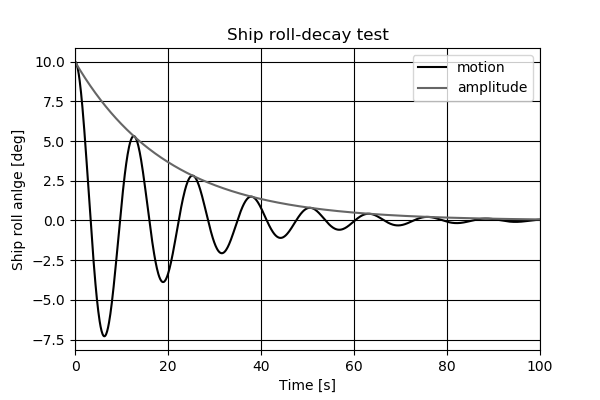
\includegraphics[width=\linewidth]{kappa/images/roll-decay.png}
    \caption{Example roll decay signal}
    \label{fig:rolldecay}
\end{figure}

\noindent The damping $B_{44}\left(\dot{\phi}\right)$ can be expressed as an expansion series:  
\begin{equation}
    B_{44}\left(\dot{\phi}\right) = B_1\cdot\dot{\phi} + B_2\cdot\dot{\phi}\left|\dot{\phi}\right| + B_3\cdot\dot{\phi}^3 + ... + B_n\cdot\dot{\phi}^n
\end{equation}
 
\noindent This series can be truncated to be expressed as a ``linear model'' (\autoref{eq:roll_decay_equation_himeno_linear}), ``quadratic model'' (\autoref{eq:roll_decay_equation_himeno_quadratic_b}), and ``cubic model'' (\autoref{eq:roll_decay_equation_cubic}).

\begin{equation} \label{eq:roll_decay_equation_himeno_linear}
A_{44} \ddot{\phi} + B_{1} \dot{\phi} + C_{1} \phi = 0
\end{equation}

\begin{equation} \label{eq:roll_decay_equation_himeno_quadratic_b}
A_{44} \ddot{\phi} + C_{1} \phi + \left(B_{1} + B_{2} \left|{\dot{\phi}}\right|\right) \dot{\phi} = 0
\end{equation}

\begin{equation} \label{eq:roll_decay_equation_cubic}
A_{44} \ddot{\phi} + \left(B_{1} + B_{2} \left|{\dot{\phi}}\right| + B_{3} \dot{\phi}^{2}\right) \dot{\phi} + \left(C_{1} + C_{3} \phi^{2} + C_{5} \phi^{4}\right) \phi = 0
\end{equation}

Models for the remaining degrees of freedom are presented in the next section.

\section{Vessel Manoeuvring Models} \label{sec:manoeuvring model}
\label{\detokenize{02.01_manoeuvring models:vessel-manoeuvring-models}}\label{\detokenize{02.01_manoeuvring models:vmm}}\label{\detokenize{02.01_manoeuvring models::doc}}
Ship manoeuvring is a simplified case of seakeeping. The encountering waves have been removed, assuming calm water conditions. The manoeuvring motions have low frequencies so that added masses and other hydrodynamic derivatives can be assumed as constants  \cite{fossen_handbook_2021}. Three manoeuvring models are used in this thesis: 
\begin{itemize}
    \item Linear (LVMM) \cite{matusiak_dynamics_2017}
    \item Abkowitz (AVMM), \cite{abkowitz_ship_1964}
    \item Modified Abkowitz (MAVMM), which is proposed in Paper \ref{pap:pit}
\end{itemize}

\noindent\autoref{\detokenize{02.01_manoeuvring models:coordinate-system}} shows the reference frames used in the manoeuvring models where \(x_0\) and \(y_0\) and heading \(\Psi\) are the global position and orientation of a ship fix reference frame \(O(x,y,z)\) (or rather \(O(x,y)\) when heave is excluded) with origin at midship. \(u\), \(v\), \(r\), \(X\), \(Y\) and \(N\) are velocities and forces in the ship fix reference frame.



\begin{figure}[H]
    \centering
    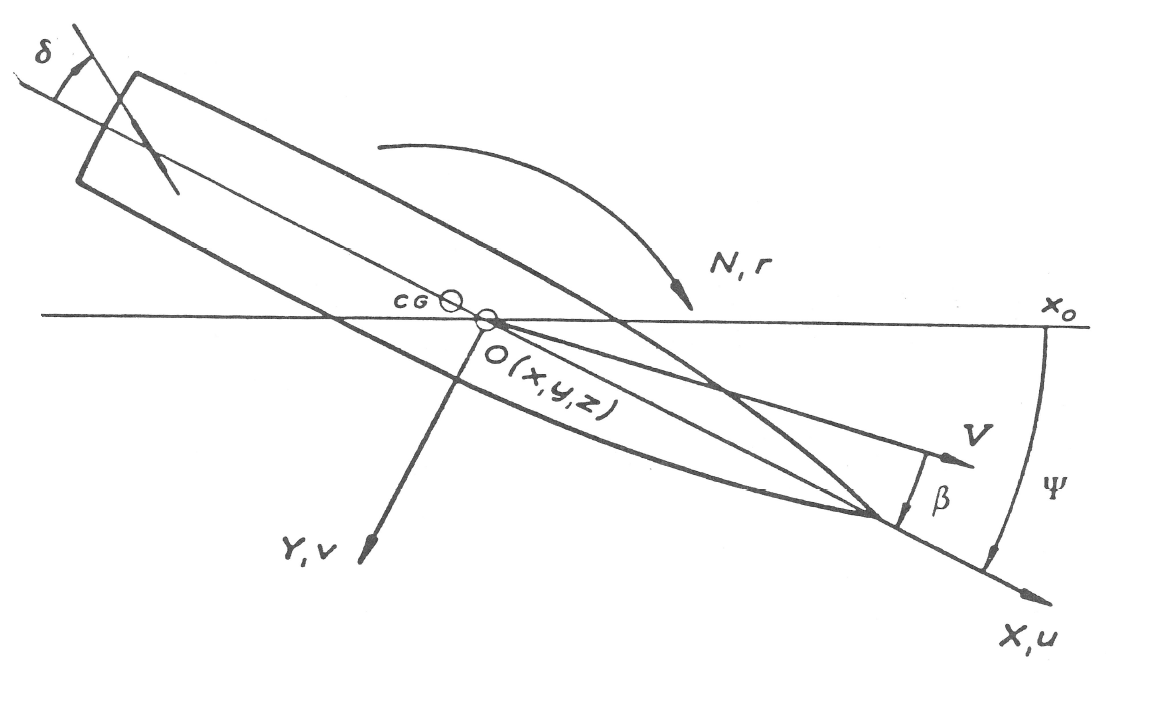
\includegraphics[width=0.8\textwidth]{kappa/images/coordinate_system.PNG}
    \caption{Reference frames.}
    \label{\detokenize{02.01_manoeuvring models:coordinate-system}}
\end{figure}

The manoeuvring equation can be described as \cite{fossen_handbook_2021},
\begin{equation}\label{equation:02.01_manoeuvring models:eqqsystem}
\begin{split}\displaystyle \left[\begin{matrix}- X_{\dot{u}} + m & 0 & 0\\0 & - Y_{\dot{v}} + m & - Y_{\dot{r}} + m x_{G}\\0 & - N_{\dot{v}} + m x_{G} & I_{z} - N_{\dot{r}}\end{matrix}\right] \left[\begin{matrix}\dot{u}\\\dot{v}\\\dot{r}\end{matrix}\right] = \left[\begin{matrix}m r^{2} x_{G} + m r v + \operatorname{X_{D}}{\left(u,v,r,\delta,thrust \right)}\\- m r u + \operatorname{Y_{D}}{\left(u,v,r,\delta,thrust \right)}\\- m r u x_{G} + \operatorname{N_{D}}{\left(u,v,r,\delta,thrust \right)}\end{matrix}\right]\end{split}
\end{equation}

\noindent where the first matrix describes the inertia of the ship in the surge, sway and yaw directions. The inertia in air is represented by the mass $m$ and moment of inertia $I_z$. The added mass in water is represented by: $X_{\dot{u}}$, $Y_{\dot{v}}$, $Y_{\dot{r}}$, $N_{\dot{v}}$ and $N_{\dot{r}}$. The hydrodynamic forces from the ship hull and rudder are desribed in the functions $X_D()$, $Y_D()$ and $N_D()$. The accelerations ($\dot{u}$, $\dot{v}$ and $\dot{r}$) can be solved from this equation,
\begin{equation}\label{equation:02.01_manoeuvring models:eqacc}
\begin{split}\displaystyle \dot{\nu} = \left[\begin{matrix}\dot{u}\\\dot{v}\\\dot{r}\end{matrix}\right] = \left[\begin{matrix}\frac{1}{- X_{\dot{u}} + m} & 0 & 0\\0 & - \frac{- I_{z} + N_{\dot{r}}}{S} & - \frac{- Y_{\dot{r}} + m x_{G}}{S}\\0 & - \frac{- N_{\dot{v}} + m x_{G}}{S} & - \frac{Y_{\dot{v}} - m}{S}\end{matrix}\right] \left[\begin{matrix}m r^{2} x_{G} + m r v + \operatorname{X_{D}}{\left(u,v,r,\delta,thrust \right)}\\- m r u + \operatorname{Y_{D}}{\left(u,v,r,\delta,thrust \right)}\\- m r u x_{G} + \operatorname{N_{D}}{\left(u,v,r,\delta,thrust \right)}\end{matrix}\right]\end{split}
\end{equation}
\sphinxAtStartPar
where \(S\) is a helper variable:
\begin{equation}\label{equation:02.01_manoeuvring models:eq_S}
\begin{split}\displaystyle S = - I_{z} Y_{\dot{v}} + I_{z} m + N_{\dot{r}} Y_{\dot{v}} - N_{\dot{r}} m - N_{\dot{v}} Y_{\dot{r}} + N_{\dot{v}} m x_{G} + Y_{\dot{r}} m x_{G} - m^{2} x_{G}^{2}\end{split}
\end{equation}
\sphinxAtStartPar

\noindent A state space model for manoeuvring can now be defined with six states:
\begin{equation}\label{equation:02.01_manoeuvring models:eq_x}
\begin{split}\displaystyle \mathbf{x} = \left[\begin{matrix}x_{0}\\y_{0}\\\Psi\\u\\v\\r\end{matrix}\right]\end{split}
\end{equation}
\noindent where $x_0$, $y_0$ and $\Psi$ are the global coordinates and heading of the ship and $u$, $v$ and $r$ are the velocities as seen in \autoref{\detokenize{02.01_manoeuvring models:coordinate-system}}.
The time derivative of this state \(\dot{\mathbf{x}}\) can be defined by a state transition \(f(\mathbf{x},\mathbf{c})\) using geometrical relations
how global coordinates \(x_0\), \(y_0\) and \(\Psi\) depend on \(u\), \(v\), and \(r\) viz.,
\begin{equation}\label{equation:02.01_manoeuvring models:eqf}
\begin{split}\displaystyle \dot{\mathbf{x}} = f(\mathbf{x},\mathbf{c}) + \mathbf{w}
                                          = \left[\begin{matrix}\dot{x_0}\\ \dot{y_0} \\ \dot{\Psi} \\\dot{u}\\\dot{v}\\\dot{r}\end{matrix}\right] + \mathbf{w}
                                          = \left[\begin{matrix}u \cos{\left(\Psi \right)} - v \sin{\left(\Psi \right)}\\u \sin{\left(\Psi \right)} + v \cos{\left(\Psi \right)}\\r\\\dot{u}\\\dot{v}\\\dot{r}\end{matrix}\right] + \mathbf{w}\end{split}
\end{equation}
\sphinxAtStartPar
where \(\mathbf{c}\) is control inputs (rudder angle \(\delta\) and thrust); the last three derivatives: \(\dot{u}\), \(\dot{v}\), \(\dot{r}\) are calculated with \autoref{equation:02.01_manoeuvring models:eqacc}.
\(\mathbf{w}\) is the process noise, i.e., the difference between the predicted state by the manoeuvring model and the true
state of the system. \(\mathbf{w}\) is unknown when the manoeuvring model is used for manoeuvre predictions and therefore normally
assumed to be zero, but it is an important factor when the manoeuvring model is used in the EKF (see \autoref{sec:datacleaning}).
The manoeuvring simulation can now be conducted by numerical integration of \autoref{equation:02.01_manoeuvring models:eqf}. The main difference between the manoeuvring model:s lies in how the hydrodynamic functions \(X_D(u,v,r,\delta,thrust)\), \(Y_D(u,v,r,\delta,thrust)\), \(N_D(u,v,r,\delta,thrust)\) are defined. These expressions are denoted in prime system ($X_D'$, $Y_D'$, $N_D'$) below for the various manoeuvring models: LVMM, AVMM and MAVMM.

{\normalfont \textbf{Linear vessel manoeuvring model (LVMM) \cite{matusiak_dynamics_2017}}}
\begin{equation}\label{equation:02.01_manoeuvring models:eqxlinear}
\begin{split}\begin{split}
\operatorname{X_{D}'}{\left(u',v',r',\delta\right)} = & X_{\delta} \delta + X_{r} r' + X_{u} u' + X_{v} v' 
\end{split}\end{split}
\end{equation}\begin{equation}\label{equation:02.01_manoeuvring models:eqylinear}
\begin{split}\begin{split}
\operatorname{Y_{D}'}{\left(u',v',r',\delta \right)} = & Y_{\delta} \delta + Y_{r} r' + Y_{u} u' + Y_{v} v' 
\end{split}\end{split}
\end{equation}\begin{equation}\label{equation:02.01_manoeuvring models:eqnlinear}
\begin{split}\begin{split}
\operatorname{N_{D}'}{\left(u',v',r',\delta \right)} = & N_{\delta} \delta + N_{r} r' + N_{u} u' + N_{v} v' 
\end{split}\end{split}
\end{equation}
\sphinxAtStartPar
{\normalfont \textbf{Abkowitz vessel manoeuvring model(AVMM) \cite{abkowitz_ship_1964}}}
\begin{equation}\label{equation:02.01_manoeuvring models:eqxabkowitz}
\begin{split}
\operatorname{X_{D}'}{\left(u',v',r',\delta,thrust' \right)} = & X_{\delta\delta} \delta^{2} + X_{r\delta} \delta r' + X_{rr} r'^{2} + X_{T} thrust' + X_{u\delta\delta} \delta^{2} u' \\ 
& + X_{ur\delta} \delta r' u' + X_{urr} r'^{2} u' + X_{uuu} u'^{3} + X_{uu} u'^{2} \\ 
& + X_{uv\delta} \delta u' v' + X_{uvr} r' u' v' + X_{uvv} u' v'^{2} \\
& + X_{u} u' + X_{v\delta} \delta v' + X_{vr} r' v' + X_{vv} v'^{2} 
\end{split}
\end{equation}

\begin{equation}\label{equation:02.01_manoeuvring models:eqyabkowitz}
\begin{split}\begin{split}
\operatorname{Y_{D}'}{\left(u',v',r',\delta,thrust' \right)} = & Y_{0uu} u'^{2} + Y_{0u} u' + Y_{0} + Y_{\delta\delta\delta} \delta^{3} + Y_{\delta} \delta + Y_{r\delta\delta} \delta^{2} r' + Y_{rr\delta} \delta r'^{2} \\ & + Y_{rrr} r'^{3} + Y_{r} r' + Y_{T\delta} \delta thrust' + Y_{T} thrust' + Y_{u\delta} \delta u' \\ & + Y_{ur} r' u' + Y_{uu\delta} \delta u'^{2} + Y_{uur} r' u'^{2} + Y_{uuv} u'^{2} v' + Y_{uv} u' v' \\ & + Y_{v\delta\delta} \delta^{2} v' + Y_{vr\delta} \delta r' v' + Y_{vrr} r'^{2} v' + Y_{vv\delta} \delta v'^{2} + Y_{vvr} r' v'^{2} \\ & + Y_{vvv} v'^{3} + Y_{v} v' 
\end{split}\end{split}
\end{equation}\begin{equation}\label{equation:02.01_manoeuvring models:eqnabkowitz}
\begin{split}\begin{split}
\operatorname{N_{D}'}{\left(u',v',r',\delta,thrust' \right)} = & N_{0uu} u'^{2} + N_{0u} u' + N_{0} + N_{\delta\delta\delta} \delta^{3} + N_{\delta} \delta + N_{r\delta\delta} \delta^{2} r' + N_{rr\delta} \delta r'^{2} \\ & + N_{rrr} r'^{3} + N_{r} r' + N_{T\delta} \delta thrust' + N_{T} thrust' + N_{u\delta} \delta u' \\ & + N_{ur} r' u' + N_{uu\delta} \delta u'^{2} + N_{uur} r' u'^{2} + N_{uuv} u'^{2} v' + N_{uv} u' v' \\ & + N_{v\delta\delta} \delta^{2} v' + N_{vr\delta} \delta r' v' + N_{vrr} r'^{2} v' + N_{vv\delta} \delta v'^{2} + N_{vvr} r' v'^{2} \\ & + N_{vvv} v'^{3} + N_{v} v' 
\end{split}\end{split}
\end{equation}
\sphinxAtStartPar
{\normalfont \textbf{Modified Abkowitz vessel manoeuvring model (MAVMM)}}
\newline
Only the most relevant coefficients in AVMM are included, as proposed in Paper \ref{pap:pit}.
\begin{equation}\label{equation:02.01_manoeuvring models:eqxmartinssimple}
\begin{split}\begin{split}
\operatorname{X_{D}'}{\left(u',v',r',\delta,thrust' \right)} = & X_{\delta\delta} \delta^{2} + X_{rr} r'^{2} + X_{T} thrust' + X_{uu} u'^{2} + X_{u} u' + X_{vr} r' v' 
\end{split}\end{split}
\end{equation}\begin{equation}\label{equation:02.01_manoeuvring models:eqymartinssimple}
\begin{split}\begin{split}
\operatorname{Y_{D}'}{\left(u',v',r',\delta,thrust' \right)} = & Y_{\delta} \delta + Y_{r} r' + Y_{T\delta} \delta thrust' + Y_{T} thrust' + Y_{ur} r' u' \\ & + Y_{u} u' + Y_{vv\delta} \delta v'^{2} + Y_{v} v' 
\end{split}\end{split}
\end{equation}\begin{equation}\label{equation:02.01_manoeuvring models:eqnmartinssimple}
\begin{split}\begin{split}
\operatorname{N_{D}'}{\left(u',v',r',\delta,thrust' \right)} = & N_{\delta} \delta + N_{r} r' + N_{T\delta} \delta thrust' + N_{T} thrust' + N_{ur} r' u' + N_{u} u' \\ & + N_{vv\delta} \delta v'^{2} + N_{v} v' 
\end{split}\end{split}
\end{equation}
\sphinxAtStartPar
The hydrodynamic functions above are expressed using nondimensional units with the prime system, denoted by the prime symbol (\('\)). The quantities are expressed in the prime system, using the denominators in Tab.\ref{tab:my_label}. For instance, surge linear velocity \(u\) can be expressed in the prime system as seen in \autoref{equation:02.01_manoeuvring models:eqprime} using the linear velocity denominator.
\begin{equation}\label{equation:02.01_manoeuvring models:eqprime}
\begin{split}\displaystyle u'=\frac{u}{V}\end{split}
\end{equation}
\sphinxAtStartPar
Equations can either be written in the prime or regular Standard Institute (SI) system. The hydrodynamic derivatives are always expressing forces in the prime system as function of state variables. The (\('\)) sign is therefore implicit and not written out as seen in \autoref{equation:02.01_manoeuvring models:eqderivativeprime}.
\begin{equation}\label{equation:02.01_manoeuvring models:eqderivativeprime}
\begin{split}\displaystyle Y_{\delta'}'=\frac{\partial Y_D'}{\partial \delta'} := Y_{\delta} \end{split}
\end{equation}
\sphinxAtStartPar
The exceptions are the added masses (\(X_{\dot{u}}\), \(Y_{\dot{v}}\), \(Y_{\dot{r}}\), \(N_{\dot{v}}\) and \(N_{\dot{r}}\)) which are expressed in both Prime system or the regular SI system where the (\('\)) sign is therefore
explicitly stated.
There is however a great benefit in expressing the hydrodynamic forces in the prime system. The forces are often nonlinear due to a quadratic relation to the flow velocity, as seen in \autoref{equation:02.01_manoeuvring models:eqquadraticsi}.
\begin{equation}\label{equation:02.01_manoeuvring models:eqquadraticsi}
\begin{split}\displaystyle Y_{D}=Y_{\delta} \cdot \delta \cdot \frac{L^2V^2\rho}{2}\end{split}
\end{equation}
which becomes linear when expressed in the prime system as seen in \autoref{equation:02.01_manoeuvring models:eqquadraticprime}.
\begin{equation}\label{equation:02.01_manoeuvring models:eqquadraticprime}
\begin{split}\displaystyle Y_{D}'=Y_{\delta} \cdot \delta'\end{split}
\end{equation}


\begin{table}[]
\caption{Prime system denominators.}
\label{tab:prime-system-denominators}
\centering
\label{tab:my_label}
\begin{tabular}{c c}
\toprule
Quantity &
Denominators
\\
\hline

angle
&

\(1\)
\\


angular
acceleration
&

\(\frac{V^{2}}{L^{2}}\)
\\


angular
velocity
&

\(\frac{V}{L}\)
\\


area
&

\(L^{2}\)
\\


density
&

\(\frac{\rho}{2}\)
\\


force
&

\(\frac{L^{2} V^{2} \rho}{2}\)
\\


frequency
&

\(\frac{V}{L}\)
\\


inertia
moment
&

\(\frac{L^{5} \rho}{2}\)
\\


length
&

\(L\)
\\


linear
acceleration
&

\(\frac{V^{2}}{L}\)
\\


linear
velocity
&

\(V\)
\\


mass
&

\(\frac{L^{3} \rho}{2}\)
\\


moment
&

\(\frac{L^{3} V^{2} \rho}{2}\)
\\


time
&

\(\frac{L}{V}\)
\\


volume
&

\(L^{3}\)
\\
\bottomrule

\end{tabular}


\end{table}

\subsection{The propeller model}
\label{\detokenize{02.10_propeller_model:the-propeller-model}}\label{\detokenize{02.10_propeller_model::doc}}

A propeller model is developed based on Manoeuvring Modeling Group (MMG) model \cite{yasukawa_introduction_2015-1} where the thrust is expressed as:
\begin{equation}\label{equation:02.10_propeller_model:eqT}
\begin{split}\displaystyle thrust = D^{4} K_{T} n^{2} \rho\end{split}
\end{equation}

and the thrust coefficient \(K_T\) is modelled as a second order polynomial:
\begin{equation}\label{equation:02.10_propeller_model:eqkt}
\begin{split}\displaystyle K_{T} = J^{2} k_{2} + J k_{1} + k_{0}\end{split}
\end{equation}

The advance ratio \(J\) is calculated as:
\begin{equation}\label{equation:02.10_propeller_model:eqJ}
\begin{split}\displaystyle J = \frac{u \left(1 - w_{p}\right)}{D n}\end{split}
\end{equation}

where \(D\) is propeller diameter, \(n\) is propeller speed and \(w_p\) is the wake fraction at an oblique inflow to the propeller from the drift angle and the yaw rate. A semi\sphinxhyphen{}empirical formula for \(w_p\) is provided in the MMG model. As an alternative, a simple polynomial is proposed in \autoref{equation:02.10_propeller_model:eqpropellermodel}.
\begin{equation}\label{equation:02.10_propeller_model:eqpropellermodel}
\begin{split}\displaystyle w_{p} = C_{1} \delta + C_{2} \delta^{2} + C_{3} \beta_{p}^{2} + C_{4} u + w_{p0}\end{split}
\end{equation}

\(w_p\) is modeled as a function of rudder angle \(\delta\), to include wake influence from the rudder and ship speed \(u\), to include a speed dependency. The influence from drift angle \(\beta\) and yaw rate \(r\) is expressed by \(\beta_p\) in \autoref{equation:02.10_propeller_model:eqbetap}.
\begin{equation}\label{equation:02.10_propeller_model:eqbetap}
\begin{split}\beta_p=\beta - \frac{r}{V} \cdot x_p \end{split}
\end{equation}

Where \(x_p\) is the propeller longitudinal position and \(w_{p0}\) is the regular Taylor wake fraction, applicable to straight ahead steaming with no rudder angle. Similar to the MMG propeller model, two sets of parameters \(C_1\)-\(C_4\) should be used in the propeller model depending on the sign of \(\beta_p\).
%%%%%%%%%%%%%%%%%%%%%%%%%%%%%%%
%%%%%%%%%%%%%%%%%%%%%%%%%%%%%%%
\chapter{Methods\label{ch:methods}}
%%%%%%%%%%%%%%%%%%%%%%%%%%%%%%%
%Section comments: There were more changes related to objective language and directional words. There is a missing term near line 13.
The system identification of rigid body ship dynamics can be simplified into parameter estimation if parameterized physical models can be assumed. Parameter estimations for roll motion and manoeuvring are presented in \ref{sec:_roll} and \ref{sec:_VMM}. System identification can be performed by selecting the most appropriate model from a collection of candidate models.

\section{Roll model parameter estimation} \label{sec:_roll}
\noindent Parameter estimation can be applied to identify the roll damping parameters ($B_1$, $B_2$, $B_3$) and stiffness parameters ($C_1$, $C_3$, $C_5$) in the parameterized roll motion models from the previous chapter (\autoref{eq:roll_decay_equation_himeno_linear}, \autoref{eq:roll_decay_equation_himeno_quadratic_b} and \autoref{eq:roll_decay_equation_cubic}). These equations do not have unique solutions because each equation can be multiplied by an arbitrary factor to obtain a new valid solution. Inertia is therefore excluded to obtain unique solutions. This is achieved by normalizing the equations by the total roll inertia $A_{44}$, as seen in Eq.\ref{eq:roll_decay_nonedim_a44}, for the linear model.

\begin{equation} \label{eq:roll_decay_nonedim_a44}
\ddot{\phi} + \frac{B_{1}}{A_{44}} \dot{\phi} + \frac{C_{1}}{A_{44}} \phi = 
\ddot{\phi} + B_{1A} \dot{\phi} + C_{1A} \phi = 0
\end{equation}

\noindent The identified normalized damping and stiffness parameters $B_{1A}$ and $C_{1A}$ can be expressed in dimensional units by multiplication with the normalization factor $A_{44}$. If $A_{44}$ is unknown before hand, it can be calculated using Eq.\ref{eq:A_44_eq} \cite{piehl_ship_2016}, assuming that the meta center height $GM$ is known.
\begin{equation} \label{eq:A_44_eq}
A_{44} = \frac{GM g m}{\omega_{0}^{2}}
\end{equation}


\noindent The frequency $\omega_0$ can be obtained with Fast Fourier transform (FFT) of the roll signal. 
Two methods have been investigated: the ``derivation approach'', referred to in \parencite{imo_1200_2006}, and the ``integration approach'' used in \cite{soder_assessment_2019}. 

\subsection{Derivation approach}\label{sec:derivation_approach}
In the derivation approach, Eq.\ref{eq:roll_decay_nonedim_a44} is treated as a linear regression problem, where the states ($\phi$, $\dot{\phi}$, $\ddot{\phi}$) are known and the parameters $B_1$ and $C_1$ must be regressed. Only roll angle $\phi$ is known from the experimental data, which means that the velocity and acceleration $\dot{\phi}$, $\ddot{\phi}$ also must be estimated (note that this is done with numerical differentiation in Paper \ref{pap:rolldamping} and with the extended Kalman filter (EKF) in Paper \ref{pap:pit}).
A least squares fit must be applied to the roll motion equation to identify the damping and stiffness parameters.

\subsection{Integration approach}\label{sec:integration_approach}
In the integration approach, Eq.\ref{eq:roll_decay_nonedim_a44} is solved as an ordinary differential equation (ODE) for many estimated sets of parameters until the solution converges. This method is time-consuming, and convergence is not guaranteed. However, the advantage is that only roll angle $\phi$ is needed.

\section{Manoeuvring model parameter estimation} \label{sec:_VMM}
In the proposed parameter estimation, a manoeuvring model is used to solve the reversed manoeuvring problem. The problem may consist of predicting unknown forces from known manoeuvring model test data. The hydrodynamic derivatives in the manoeuvring model can be identified through regression of the force polynomials on forces predicted with inverse dynamics (see \autoref{\detokenize{03.01_inverse_dynamics::doc}}).
The measurement noise must be removed prior to the regression of hydrodynamic derivatives in the manoeuvring model. This is conducted by an extended Kalman filter (EKF) and a Rauch Tung Striebel (RTS) smoother (see \autoref{sec:datacleaning}). The EKF requires an accurate manoeuvring model as the predictor.
Therefore, the accurate manoeuvring model is both the input and output of the method. A linear manoeuvring model that includes hydrodynamic derivatives estimated with semi-empirical formulas (\autoref{app:initial_estimates}) is used as the initial predictor. Once the regressed manoeuvring model has been obtained, the parameter estimation can be refined, using the regressed manoeuvring model as the predictor model in the EKF, to improve the filter and obtain a more accurate manoeuvring model. The method is summarized in Fig.\ref{fig:greyvmm} and can be repeated several times (indicated by the dashed arrow) for improved accuracy. 

\begin{figure}[H]
    
    \centering
    \begin{tikzpicture}[node distance=1.5cm]
    %\draw (0,0) rectangle (10,10); %create a bounding box to reserve space
    \node (data) [io] {\footnotesize Model test data: $x$, $\delta$, thrust};
    
    \node (EKF) [process, right of=data, xshift=3.0cm] {\footnotesize EFK + RTS};
    \node (predictor) [process, right of=EKF, xshift=2.0cm]{\footnotesize Predictor};
    \node (VMM) [io, right of=predictor, xshift=1.0cm] {\footnotesize initial model};
    
    \node (data_clean) [io, below of=EKF] {\footnotesize \(x,\dot{x},\ddot{x}, \delta, thrust\)};
    
    \node (black-box) [black-box, below of=data_clean] {\footnotesize Regression};
    
    \node (X_D) [io, left of=black-box, xshift=-0.70cm, yshift=0.7cm]{\footnotesize \(X_D\)};
    \node (Y_D) [io, left of=black-box, xshift=-0.70cm, yshift=0cm]{\footnotesize \(Y_D\)};
    \node (N_D) [io, left of=black-box, xshift=-0.70cm, yshift=-0.7cm]{\footnotesize \(N_D\)};
    
    \node (white-box) [white-box, left of=Y_D, xshift=-1.00cm] {\footnotesize Inverse dynamics};
    
    
    %
    %
    \node (coefficients) [io, right of=black-box, xshift=2.0cm] {\footnotesize model$\left(Y_{uv},N_{\delta},...\right)$};
    
    \draw [arrow] (data) -- (EKF);
    \draw [arrow] (predictor) -- (EKF);
    \draw [arrow] (VMM) -- (predictor);
    \draw [arrow] (EKF) -- (data_clean);
    
    \draw [arrow] (data_clean) -| (white-box);
    \draw [arrow] (data_clean) -- (black-box);
    
    \draw [arrow] (white-box) -- (X_D);
    \draw [arrow] (white-box) -- (Y_D);
    \draw [arrow] (white-box) -- (N_D);
    
    \draw [arrow, shorten >=0.5cm] (X_D) -- (black-box);
    \draw [arrow, shorten >=0.2cm] (Y_D)  -- (black-box);
    \draw [arrow, shorten >=0.5cm] (N_D)  -- (black-box);
    
    \draw [arrow] (black-box)  -- (coefficients);
    \draw [arrow, dashed] (coefficients)  -- (predictor);
    
    \end{tikzpicture}
    \caption{Method to estimate the manoeuvring model hydrodynamic derivatives}
    \label{fig:greyvmm}
\end{figure}

\noindent Using semi-empirical formulas (\autoref{app:initial_estimates}) for the initially estimated manoeuvring model adds prior knowledge about the ship dynamics to the regression. An example, with simulation results from the steps in the iteration, is presented in \hyperref[\detokenize{01.01_method:iterations}]{Fig.\@\ref{\detokenize{01.01_method:iterations}}}.


\begin{figure}[H]
    \centering
    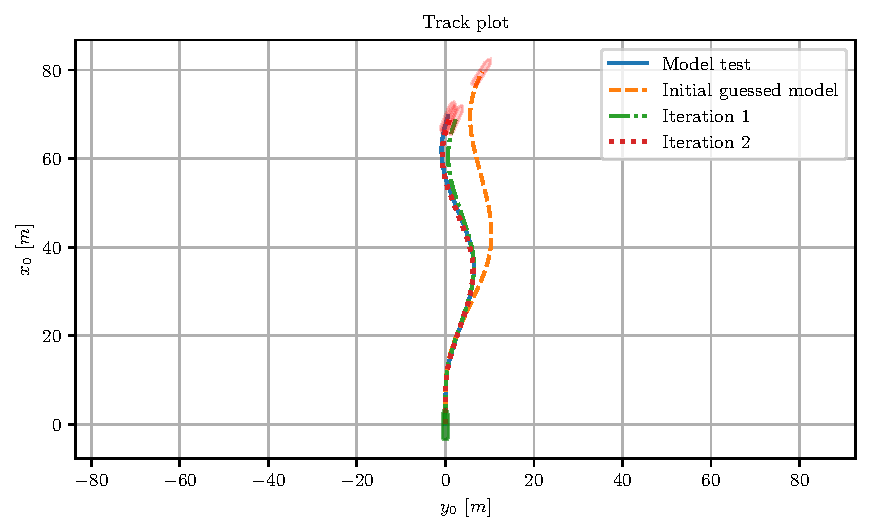
\includegraphics[width=\textwidth]{kappa/images/0.pdf}
    \caption{Simulation with: initial model and first and second iteration of the parameter estimation method.}
    \label{\detokenize{01.01_method:iterations}}
\end{figure}

\subsection{Inverse dynamics and regression}
\label{\detokenize{03.01_inverse_dynamics:inverse-dynamics-and-regression}}\label{\detokenize{03.01_inverse_dynamics::doc}}

Each manoeuvring model has some hydrodynamic functions \(X_D(u,v,r,\delta,thrust)\), \(Y_D(u,v,r,\delta,thrust)\), \(N_D(u,v,r,\delta,thrust)\) that are defined as polynomials. The hydrodynamic derivatives in these polynomials can be identified with force regression of measured forces and moments. The measured forces and moments are usually taken from captive model tests (CMT), planar motion mechanism (PMM) tests, or virtual captive tests (VCT). However, motions are recorded when the ship is free in all degrees of freedom. Hence, forces and moments causing ship motion must be estimated by solving the inverse dynamics problem.
The inverse dynamics problem is solved by restructuring the system equation (\autoref{equation:02.01_manoeuvring models:eqacc}) to get the hydrodynamics functions on the left-hand side. If the mass and inertia of the ship with added masses: \(X_{\dot{u}}\), \(Y_{\dot{v}}\), \(Y_{\dot{r}}\), \(N_{\dot{v}}\), and \(N_{\dot{r}}\) are known; the forces in the Prime system can be calculated using \autoref{equation:03.01_inverse_dynamics:eqxd}, \autoref{equation:03.01_inverse_dynamics:eqyd}, and \autoref{equation:03.01_inverse_dynamics:eqnd}.
These forces can be used to regress the hydrodynamic derivatives through the ordinary least square (OLS) method. If the added masses are unknown, they can be calculated using potential flow methods or semi-empirical methods (\autoref{app:initial_estimates}). 
\begin{equation}\label{equation:03.01_inverse_dynamics:eqxd}
\begin{split}\displaystyle \operatorname{X_{D}'}{\left(u',v',r',\delta,thrust' \right)} = - X_{\dot{u}}' \dot{u}' + \dot{u}' m' - m' r'^{2} x_{G}' - m' r' v'\end{split}
\end{equation}\begin{equation}\label{equation:03.01_inverse_dynamics:eqyd}
\begin{split}\displaystyle \operatorname{Y_{D}'}{\left(u',v',r',\delta,thrust' \right)} = - Y_{\dot{r}}' \dot{r}' - Y_{\dot{v}}' \dot{v}' + \dot{r}' m' x_{G}' + \dot{v}' m' + m' r' u'\end{split}
\end{equation}\begin{equation}\label{equation:03.01_inverse_dynamics:eqnd}
\begin{split}\displaystyle \operatorname{N_{D}'}{\left(u',v',r',\delta,thrust' \right)} = I_{z}' \dot{r}' - N_{\dot{r}}' \dot{r}' - N_{\dot{v}}' \dot{v}' + \dot{v}' m' x_{G}' + m' r' u' x_{G}'\end{split}
\end{equation}

\noindent An example that includes forces calculated with inverse dynamics from motions in a turning circle test can be seen in \hyperref[\detokenize{03.01_inverse_dynamics:fig-inverse}]{Fig.\@ \ref{\detokenize{03.01_inverse_dynamics:fig-inverse}}}. The forces have been converted to SI units.

\begin{figure}[H]
    \centering
    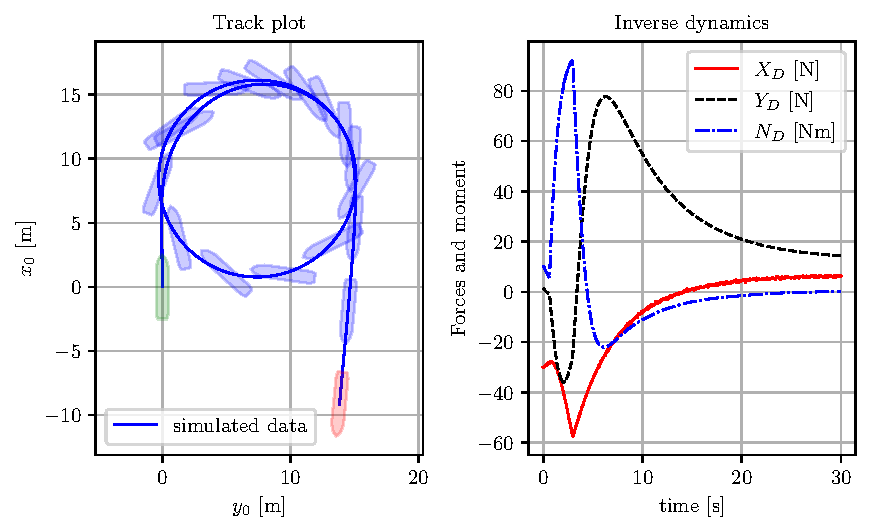
\includegraphics[width=\textwidth]{kappa/images/1.pdf}
    \caption{Forces and moments calculated with inverse dynamics on data from a turning circle test.}
    \label{\detokenize{03.01_inverse_dynamics:fig-inverse}}
\end{figure}

\subsection{Data cleaning}
\label{sec:datacleaning}
It is possible to do an exact parameter estimation on flawless (simulated) data with no noise (see Paper \ref{pap:pit}). However, such data from physical experiments does not exist in reality. The measured data will always contain process noise and measurement noise. In order to mitigate the effects of noise, the data is pre-processed using the extended Kalman filter (EKF) \cite{brown_introduction_1997} and the Rauch Tung Striebel (RTS) smoother \cite{rauch_maximum_1965}, which are both presented below.
EKF is an extension of the Kalman filter (KF) that is used to work on nonlinear systems such as the manoeuvring models. The premise is that noise can be neglected if it has no rational physical explanation. For instance, if noisy measurement data would be  completely correct, that would mean that large ship vibrations must have originated from large high frequency forces considering the large mass of the ship. A prior understanding of the dynamics suggests that these forces are not present. Therefore, the noise should be considered as measurement noise and should be removed. Low-pass filtering is commonly used to remove noise; motions above a cutoff frequency are considered unphysical measurement noise. The problem with low-pass filtering is that choosing the cutoff frequency is difficult. It is often  either too low (removing some of the signal) or too high (keeping some unfiltered measurement noise in the data). The Kalman filter has a predictor model, a manoeuvring model in this case, that continuously estimates the system’s state that runs parallel with the measurement data. The filter estimates the current state as a combination of the measurement data and the predictor model estimate based on the possible validity of the data and the model. If the data has low noise, the estimate is closer to that data. Conversely, if the model provides very accurate predictions, then that estimate is closer to the model.
The system’s inverse dynamics require everything about the state (positions, velocities, and accelerations) to be known. Only positions are known from the measurements, but the velocities and accelerations are instead estimated by the EKF.
The EKF is recursive and can be ran online; it continuously makes new estimates as new measurements arrive. The EKF uses passed measurements to estimate states in the near future. This property is commonly used for online applications such as autopilots or autonomous ships. This restriction is unnecessary for the estimation for already existing data, where an entire time series of existing measurements is available. The knowledge of both past and future data can be used to improve the filter. An EKF filter can include future time steps by adding the RTS smoother after the filter. The RTS smoother is an algorithm that runs the EKF backward to account for future time steps.

\subsection{Regression}
Finding the hydrodynamic derivatives can be defined as a linear regression problem:
\begin{equation}\label{equation:03.01_inverse_dynamics:eqregression}
\begin{split}y = X\gamma + \epsilon\end{split}
\end{equation}

\noindent A model for the hydrodynamic forces must first be assumed.
The label vector \(y\) and feature matrix \(X\) in the regression problem in \autoref{equation:03.01_inverse_dynamics:eqregression} can now be calculated based on the assumed model. For example: the label in the regression of the surge degree of freedom for the MAVMM can be calculated using the inverse dynamics force, which is expressed with primed units:
\begin{equation}\label{equation:03.01_inverse_dynamics:diff_eq_X_y}
\begin{split}\displaystyle y = - X_{\dot{u}} \dot{u}' + \dot{u}' m' - m' r'^{2} x_{G'} - m' r' v'\end{split}
\end{equation}

\noindent The feature matrix \(X\) is expressed as:
\begin{equation}\label{equation:03.01_inverse_dynamics:diff_eq_X_X}
\begin{split}\displaystyle X = \left[\begin{matrix}thrust' & u' & \delta^{2} & r'^{2} & u'^{2} & r' v'\end{matrix}\right]\end{split}
\end{equation}

\noindent The regressed hydrodynamic derivatives are stored in the \(\gamma\) vector:
\begin{equation}\label{equation:03.01_inverse_dynamics:diff_eq_X_beta}
\begin{split}\displaystyle \gamma = \left[\begin{matrix}X_{T}\\X_{u}\\X_{\delta\delta}\\X_{rr}\\X_{uu}\\X_{vr}\end{matrix}\right]\end{split}
\end{equation}

\noindent The hydrodynamic derivatives in the manoeuvring model are treated as Gaussian random variables when conducting the ordinary least squares (OLS) regression. The hydrodynamic derivatives in the manoeuvring model are usually taken as the mean value of each regressed random variable, which is the most likely estimate. The regression result can be expressed with a multivariate Gaussian distribution, which is defined by the regression’s mean values and covariance matrix. The multivariate Gaussian distribution can be used to conduct Monte Carlo simulations in the study of alternative realizations of the regression.


Strong multicollinearity is a documented problem for the manoeuvring models \cite{luo_parameter_2016}, \cite{wang_quantifying_2018}.
The thrust coefficient \(X_T\) in the hydrodynamic function \(X_D\) in \autoref{equation:02.01_manoeuvring models:eqxabkowitz} introduces multicollinearity to the regression. This coefficient can instead be calculated from the thrust deduction factor \(t_{df}\):
\begin{equation}\label{equation:03.01_inverse_dynamics:eqXthrust}
\begin{split}\displaystyle X_{T} = 1 - t_{df}\end{split}
\end{equation}

\noindent The \(X_T\) coefficient is excluded from the regression by moving it to the left-hand side of the regression equation \autoref{equation:03.01_inverse_dynamics:eqregression}:
\begin{equation}\label{equation:03.01_inverse_dynamics:eqexclude}
\begin{split}y-X_T \cdot thrust = X \gamma + \epsilon\end{split}
\end{equation}

\noindent Rudder coefficients (\(Y_R\)) from \(Y_D\) equation \autoref{equation:02.01_manoeuvring models:eqyabkowitz}, such as \(Y_{\delta}\) and \(Y_{\delta T}\), have also been excluded by assuming a connection with their \(N_D\) equation counterpart through the rudder lever arm \(x_r\):
\begin{equation}\label{equation:03.01_inverse_dynamics:eqyr}
\begin{split}\displaystyle Y_{R} = \frac{N_{R}}{x_{r'}}\end{split}
\end{equation}

\subsection{Model development process}
\label{sec:model_development_process}
The aim of developing a manoeuvring model with parameter estimation is to develop a model that can generalize outside the known data. The method presented in this thesis is assessed with the hold-out evaluation \cite{sammut_holdout_2017}. The data in this evaluation is divided into three sets: the training set, the validation set, and the test set. The development process can be seen in \autoref{fig:model_development_process}.

\begin{figure}[H]
\centering
\begin{tikzpicture}

\node (dataset)[rectangle,
    anchor=west,
    draw,
    text = black,
    minimum width=12cm,
    fill = white] at (0, 0) {\footnotesize DATASET};

\node (train)[rectangle,
    draw,
    anchor=west,
    text = black,
    minimum width=6cm,
    fill = yellow] at (0, -1cm) {\footnotesize TRAIN};

\node (validation)[rectangle,
    draw,
    anchor=west,
    text = blue,
    minimum width=3cm,
    fill = white] at (6cm, -1cm) {\footnotesize VALIDATION};

\node (test)[rectangle,
    draw,
    anchor=west,
    text = white,
    minimum width=3cm,
    fill = black!15!green!255] at (9cm, -1cm){\footnotesize TEST};
    
\node (train_multiple)[rectangle,
    draw,
    anchor=west,
    text = black,
    draw = none,
    fill = none] at (0.2cm, -2cm){\footnotesize Train candidate models};
    
\node (validate_models)[rectangle,
    draw,
    anchor=west,
    text = black,
    draw = none,
    fill = none] at (4.9cm, -2cm){\footnotesize Validate models};
    
\node (evaluate_models)[rectangle,
    draw,
    anchor=west,
    text = black,
    draw = none,
    fill = none] at (8.3cm, -2cm) {\footnotesize Evaluate final model};

\draw[->] (3,-1.3) -- (3,-1.8);
\draw[->] (7,-1.3) -- (7,-1.8);
\draw[->] (10,-1.3) -- (10,-1.8);



\end{tikzpicture}
\caption{Model development process with hold-out evaluation}
\label{fig:model_development_process}
\end{figure}

\noindent The purpose of the training set is to train all the candidate models using the proposed parameter estimation method. The validation set is then used to select the most effective candidate model. The training and validation sets are then joined to train the selected model as the final model. The final model is used for predicting the test set, which is used to evaluate the accuracy of the model. These three sets are not divided randomly;  they are divided to assess the model’s extrapolation ability. The data sets are therefore split to have the smallest yaw rates, drift-angles, and rudder-angles in the training set; the medium values in the validation set; and the largest values in the test set, which can be seen in \autoref{fig:wpcc_datasets} in the next chapter.



%%%%%%%%%%%%%%%%%%%%%%%%%%%%%%%
%%%%%%%%%%%%%%%%%%%%%%%%%%%%%%%
\chapter{Results\label{ch:results}}
%%%%%%%%%%%%%%%%%%%%%%%%%%%%%%%
This chapter presents a summary of the appended papers, including research activities
and a selection of the important results, and highlights the main achievements. A model for the roll motion is developed in Paper \ref{pap:rolldamping}. A manoeuvring model is developed in Paper \ref{pap:daiyong} and Paper \ref{pap:pit} and the model generalization is addressed in Paper \ref{pap:pit}.

\section{Summary of Paper \ref{pap:rolldamping}}
\subsection*{"\nameref{pap:rolldamping}"}
System identification of ship roll motion, including roll damping and stiffness, is developed in in Paper \ref{pap:rolldamping}. In the second generation of intact stability criteria, the IMO addressed the importance of ships having sufficient roll damping to avoid large roll motions, parametric rolling, and excessive acceleration \parencite{imo_finalization_2016}. These phenomena have been well known for a very long time. Parametric roll was observed already by \parencite{froude_rolling_1861} and has been on the agenda of the marine research community since the early 1950s \parencite{galeazzi_early_2013}; it has received much more attention since \parencite{france_investigation_2001} showed that the APL China casualty in 1998, where a post-Panamax C11 class container ship lost almost a third of its containers, was most likely caused by head sea parametric rolling. The damping of roll motion plays an important part during the above-mentioned phenomena. It has been shown that the relatively small difference in the roll damping prediction they obtained with small method variation, could mean the difference between severe roll angles and hardly noticeable motions \parencite{soder_ikeda_2019}.

The objective in Paper \ref{pap:rolldamping} was therefore to improve the roll damping predictions for modern ships. The roll damping was studied using time series data from 250 (see Fig. \ref{fig:ship_types}) roll decay tests (see \autoref{sec:roll}) assembled from the Maritime Dynamics Laboratory at SSPA Sweden AB (\href{www.sspa.se}{www.sspa.se}).

\begin{figure}[H]
    \centering
    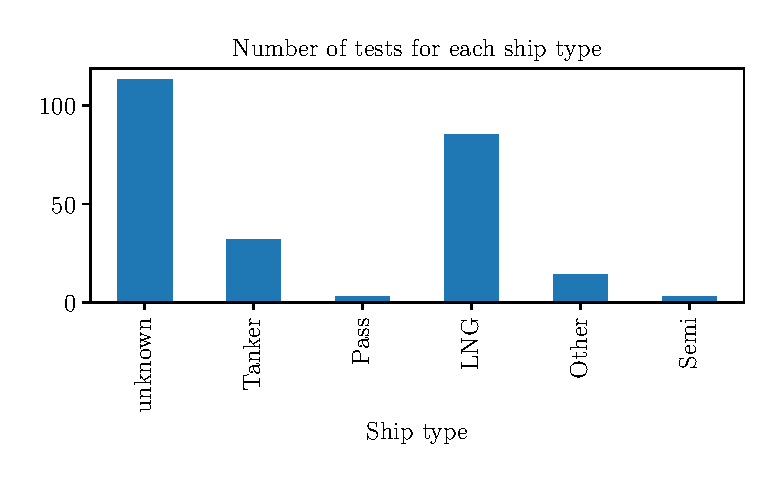
\includegraphics[width=0.5\columnwidth]{kappa/images/ship_types.eps}
    \caption{Number of tests per ship type}
    \label{fig:ship_types}
\end{figure}

\noindent The work was broken down to the following subtasks: 
\begin{itemize}
    \item Find the mathematical model that best describes the roll motion
    \item Identify the parameters in this model for all the tests
    \item Develop a generic roll damping model for all ships, using those parameters
    \begin{itemize}
        \item Grey-box model
        \item Black-box model
    \end{itemize}
\end{itemize}

\noindent The work is also summarized in \autoref{fig:paper1_overview}. System identification on the time series from the roll decay database was performed with the linear (\autoref{eq:roll_decay_equation_himeno_linear}), quadratic (\autoref{eq:roll_decay_equation_himeno_quadratic_b}) and cubic model (\autoref{eq:roll_decay_equation_cubic}). Roll damping parameters identified from the model that was found to be the best was used to build a roll damping database. The identified roll dampings could then be compared with corresponding predictions with the Simplified-Ikedas method \cite{kawahara_simple_2011}, being the state of art prediction for ship roll damping.
The generic roll damping model was then developed as a grey-box model, including the Simplified-Ikedas method as the white part, and a pure black-box model.
\begin{figure}[H]
    \centering
    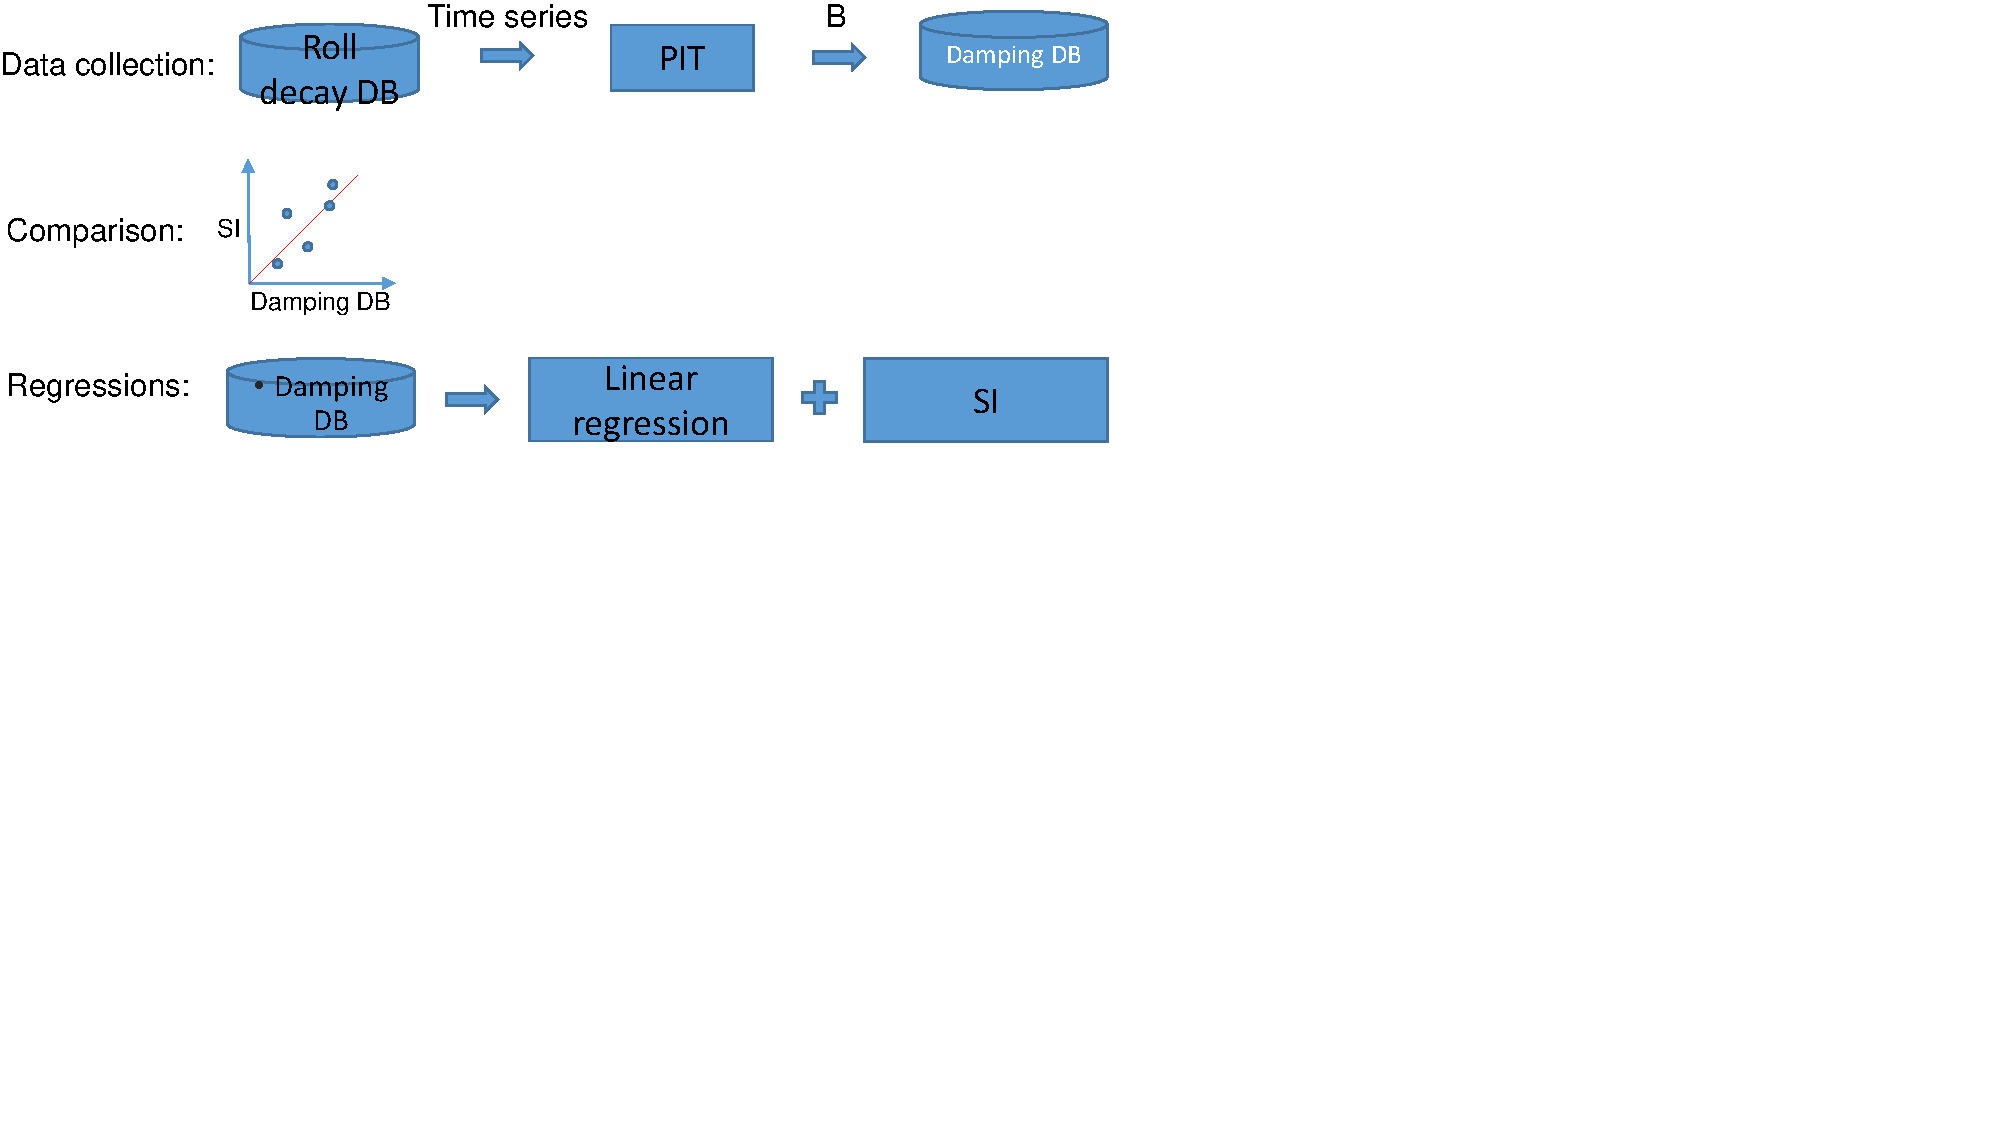
\includegraphics[width=\linewidth]{kappa/images/workflow.pdf}
    \caption{Overview of the work conducted for Paper \ref{pap:rolldamping}}
    \label{fig:paper1_overview}
\end{figure}

\subsection{Best mathematical model for the roll motion}
System identification on the linear, quadratic and cubic model was conducted using both the ''integration approach'' (described in \autoref{sec:integration_approach}) and the ''derivation approach'' (described in \autoref{sec:derivation_approach}).
Results from simulations with the identified models is shown for one of the roll-decay tests in \autoref{fig:roll_decay_compare}.

\begin{figure}[H]
    \centering
    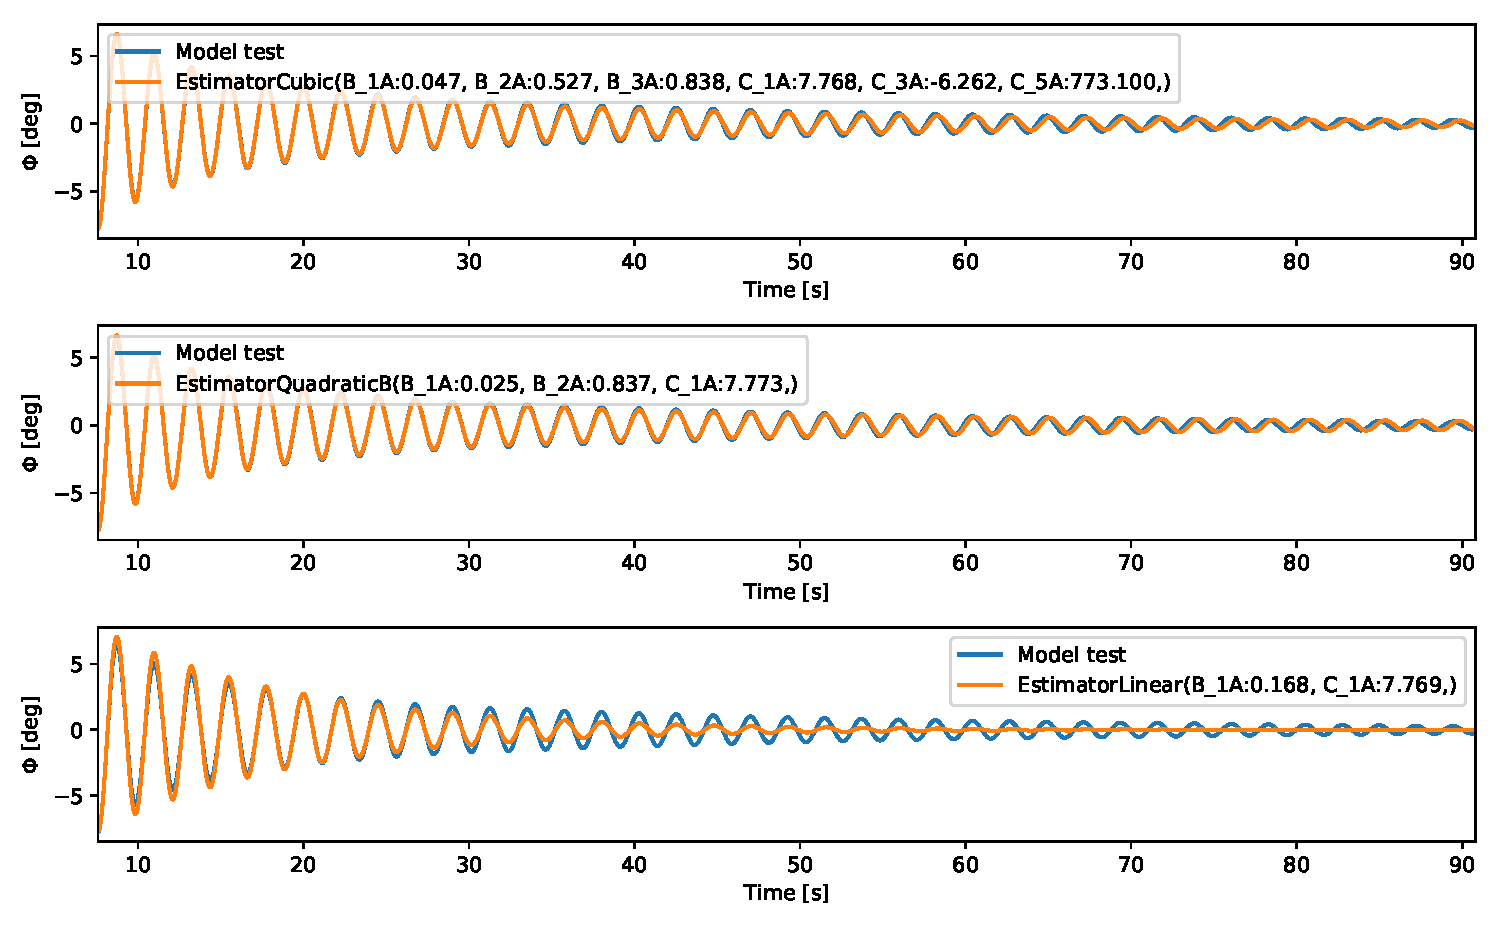
\includegraphics{kappa/images/roll_decay_model_compare.pdf}
    \caption{Caption}
    \label{fig:roll_decay_compare}
\end{figure}

\subsection{Generic roll damping model}
\label{sec:genericrolldampingmodel}
A serial grey-box model for ship roll damping (see Fig.\ref{fig:greyrolldamping}) is also developed in Paper \ref{pap:rolldamping}. 
This is expanding the system identification, not only focusing on one ship, but rather all modern ships, by a prediction model of the damping coefficients from the  applied on a whole database of roll decay tests. 
Simplified Ikeda's method \cite{kawahara_simple_2011} is used as the white box model, which is combined with a following black-box correction model.

\begin{figure}[H]
    
    \centering
    \begin{tikzpicture}[node distance=2cm]
    \node (white-box) [white-box] {Simplified Ikeda};
    \node (B_BK) [io, right of=white-box, xshift=0.90cm, yshift=1.5cm] {$\hat{B_{BK}}$};
    \node (B_E) [io, right of=white-box, xshift=0.75cm, yshift=0.75cm] {$\hat{B_{E}}$};
    \node (B_F) [io, right of=white-box, xshift=0.75cm, yshift=0cm] {$\hat{B_{F}}$};
    \node (B_L) [io, right of=white-box, xshift=0.75cm, yshift=-0.75cm] {$\hat{B_{L}}$};
    \node (B_W) [io, right of=white-box, xshift=0.75cm, yshift=-1.5cm] {$\hat{B_{W}}$};
    
    
    \node (black-box) [black-box, right of=B_F, xshift=0.75cm] {Black-box};
    \draw [arrow] (white-box) -- (B_BK);
    \draw [arrow] (white-box) -- (B_E);
    \draw [arrow] (white-box) -- (B_F);
    \draw [arrow] (white-box) -- (B_L);
    \draw [arrow] (white-box) -- (B_W);
    
    \draw [arrow] (B_BK) -- (black-box);
    \draw [arrow] (B_E)  -- (black-box);
    \draw [arrow] (B_F)  -- (black-box);
    \draw [arrow] (B_L)  -- (black-box);
    \draw [arrow] (B_W)  -- (black-box);
    
    
    \node (B) [io, right of=black-box, xshift=0.75cm, yshift=0cm] {$B$};
    \draw [arrow] (black-box)  -- (B);
    
    \end{tikzpicture}
    \caption{Grey-box model to predict roll damping}
    \label{fig:greyrolldamping}
\end{figure}

\noindent The roll damping data set, obtained from the roll motion investigation, is used to train the black-box part of the grey-box model. The black-box correction model of the output components from the Simplified Ikeda's method are shown in (Eq.\ref{eq:polynom_correction}),
\begin{equation} \label{eq:polynom_correction}
\hat{B_{e}} = 1.106 \hat{B_{BK}} - 0.9124 \hat{B_{E}} + 4.282 \hat{B_{F}} + 0.7457 \hat{B_{L}} + 0.1844 \hat{B_{W}} + 0.004999 \phi_{a} - 0.0005097
\end{equation}


\noindent Large corrections of the skin friction damping $\hat{B_F}$ and wave damping $\hat{B_W}$ are suggested by this expression. This is because the Simplified Ikeda's method is not very accurate for this dataset, where most of the ships in the dataset exceed the limits of the method. A pure black-box model is also devloped in Paper \ref{pap:rolldamping} (see Eq.\ref{eq:polynom_complex}),
\begin{equation} \label{eq:polynom_complex}
\begin{aligned} 
 \hat{B_{e}} = - 0.02578 A_{0} V - 0.02705 BK_{B} V + \\ 
 0.008993 BK_{L} V - 0.03191 C_{b} V - 0.2028 OG V + \\ 
 0.003472 V^{2} + \\ 
 0.004234 V \hat{\omega_{0}} - 0.002591 V \phi_{a} - 0.008384 V beam + \\ 
 0.05048 V + \\ 
 0.007814 \hat{\omega_{0}}^{2} + \\ 
 0.03882 \hat{\omega_{0}} \phi_{a} - 0.001069 \\ 
 \end{aligned}
\end{equation}


\noindent The grey-box model and the black-box model above, have about the same accuracy when performing cross-validation on the roll damping dataset. The linearized equivalent damping $B_e$ is calculated with \autoref{eq:B_e_equation} \cite{himeno_prediction_1981}. The damping and frequency is nondimensionalized with \autoref{eq:be_eqvalent} and \autoref{eq:omega0_hat_equation} \cite{himeno_prediction_1981}.

\begin{equation} \label{eq:B_e_equation}
B_{e} = B_{1} + \frac{8 B_{2} \omega_{0} \phi_{a}}{3 \pi}
\end{equation}


\begin{equation} \label{eq:be_eqvalent}
    \hat{B_e} = \frac{B_e}{\rho \bigtriangledown Beam^2} \sqrt{\frac{Beam}{2g}},
\end{equation}

\begin{equation} \label{eq:omega0_hat_equation}
\omega_{hat} = \frac{\sqrt{2} \omega_{0} \sqrt{\frac{beam}{g}}}{2}
\end{equation}


\section{Summary of Paper \ref{pap:daiyong}}
\subsection*{"\nameref{pap:daiyong}"}
Least Square Support Vector Regression (LS-SVR) \cite{brereton_support_2010} is used in Paper \ref{pap:daiyong} to identify the parameters in the AVMM.  
The data is taken from experimental tests on a lake using a ship model with a scale of 50:1. The configuration of sensors and equipment for the experiment is shown in Fig.\ref{fig:cthmodel}.  
\begin{figure}[H]
    \centering
    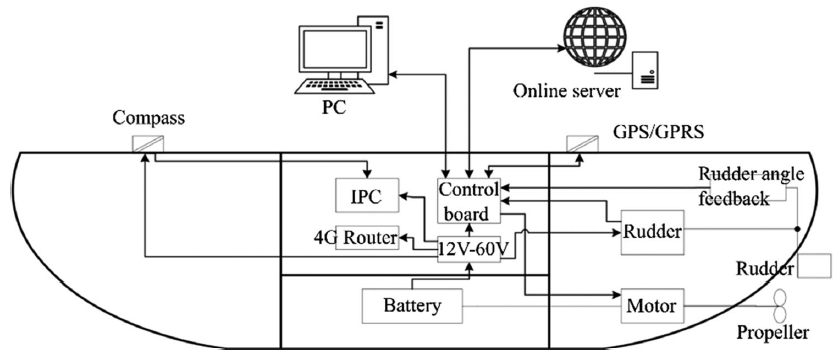
\includegraphics[width=\textwidth]{kappa/images/cth_model.png}
    \caption{Configuration of sensors and equipment for the experimental tests.}
    \label{fig:cthmodel}
\end{figure}
\noindent The hydrodynamic derivatives of the AVMM are identified almost perfectly when applied on data from simulations with MSS toolbox Mariner \cite{tristan_matlab_2009}. The  does however not work at all when applied on the data obtained from the lake experiments as seen in Fig.\ref{fig:daiyong_extrapolation}. 

\begin{figure}[H]
    \centering
    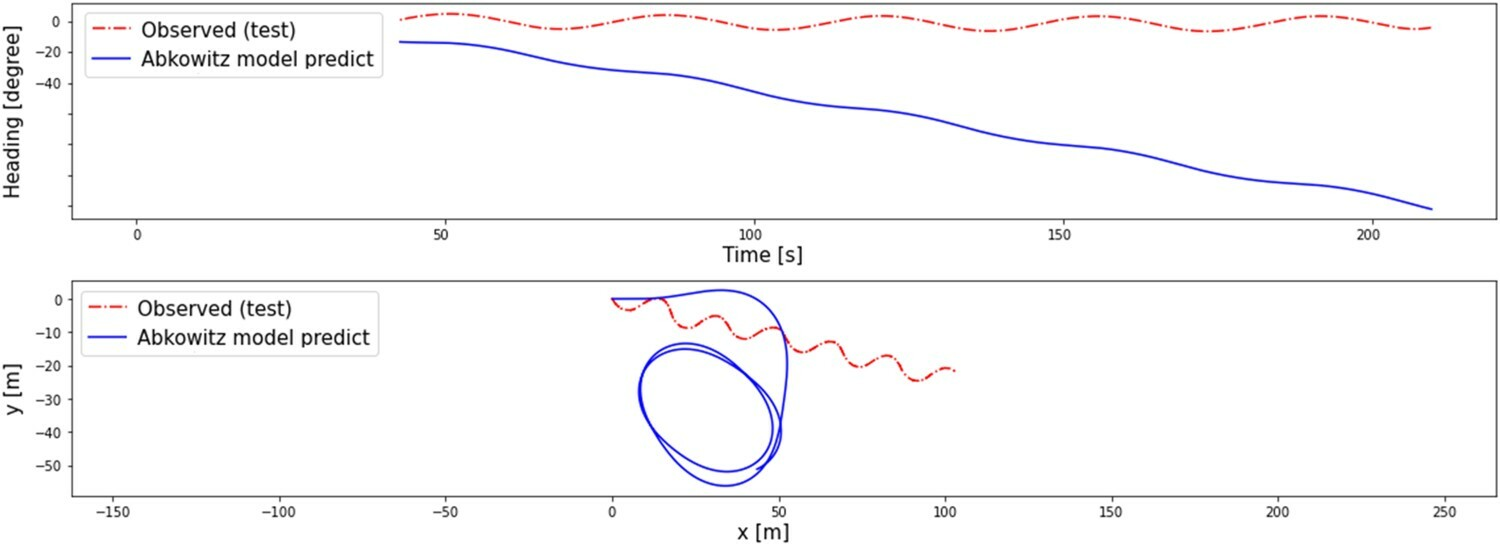
\includegraphics[width=\linewidth]{kappa/images/daiyong_extrapolation.jpeg}
    \caption{Prediction with AVMM of zigzag lake experiments.}
    \label{fig:daiyong_extrapolation}
\end{figure}

\noindent The  is very sensitive to noise due to the differentiation that needs to be conducted to calculate velocities and yaw rate from the measured position and heading. The  works better if the data is first cleaned using a proposed preprocessing algorithm together with a Kalman Filter (KF). The simulations with the identified model and the experiments were however still not in very good agreement.     

\section{Summary of Paper \ref{pap:pit}}
\subsection*{"\nameref{pap:pit}"}
A new method for System Identification of ship manoeuvring dynamics is developed in Paper \ref{pap:pit}. The system model for the ship manoeuvring is assumed to be represented by a manoeuvring model (see Section \ref{sec:manoeuvring model}). The appropriate manoeuvring model for the specific ship and data is selected from a set of candidate VMMs, with varying complexity as a function of its number of hydrodynamic derivatives. The appropriate manoeuvring model is selected to give a robust model that can make predictions outside the domain covered by the available training data. A cross validation scheme is proposed to be used in the selection. In this scheme, the validation set has larger drift angles, yaw rates and rudder angles compared to the training set as seen in the example in Fig.\ref{fig:cross_validation}.
\begin{figure}[H]
    \centering
    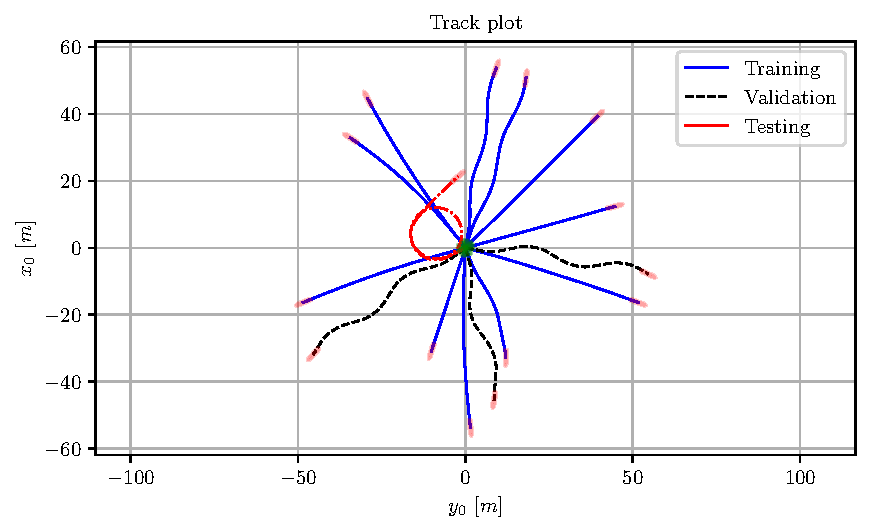
\includegraphics[width=\linewidth]{kappa/images/3.pdf}
    \caption{wPCC training, validation and testing datasets.}
    \label{fig:cross_validation}
\end{figure}
\noindent A new  for VMMs (see Section \ref{sec:_VMM}), with large focus on the data cleaning, is also proposed in Paper \ref{pap:pit}. This  is investigated together with the method to select a appropriate and robust manoeuvring model for two very different cases. The wPCC test case which is a twin screw Pure Car Truck Carrier and the KVLCC2 being a single screw Very Large Crude Carrier.    
\begin{itemize}
    
    \item It is shown that the hydrodynamic derivatives within a manoeuvring model can be identified exactly at ideal conditions with no measurement noise and a perfect estimator.
    
    \item It is shown that the proposed prepossessing of measurement data with EKF + RTS run in iteration with initial guess from semi-empirical formulas, is better than using low-pass filters for cleaning. \autoref{fig:lowpass-accuracy} shows the average simulation error with the  using various low-pass filters or the EKF + RTS smoother.
    \begin{figure}[h]
        \centering
        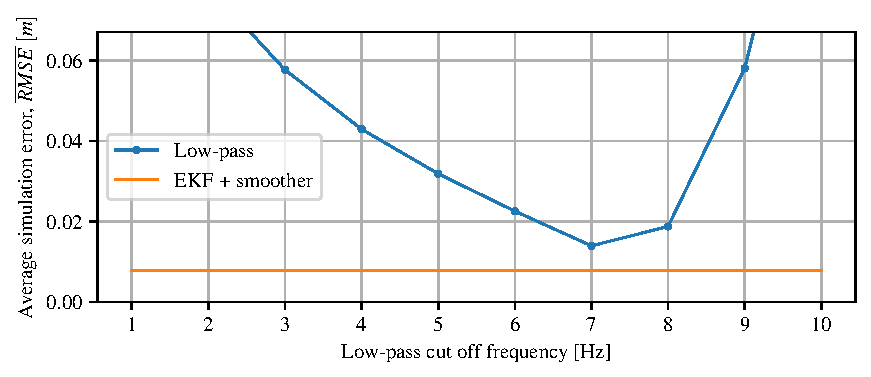
\includegraphics{kappa/images/6.pdf}
        \caption{Average simulation error with MAVMM fitted on wPCC model test data using low-pass filters with various cutt off frequency or EKF.}
        \label{fig:lowpass-accuracy}
    \end{figure}
    
    \item The  has large problems with multicollinearity for the AVMM. The absolute correction between the features is shown in \autoref{fig:ncorr}. This was less of a problem for the less complex model MAVMM.
    \begin{figure}[h]
        \centering
        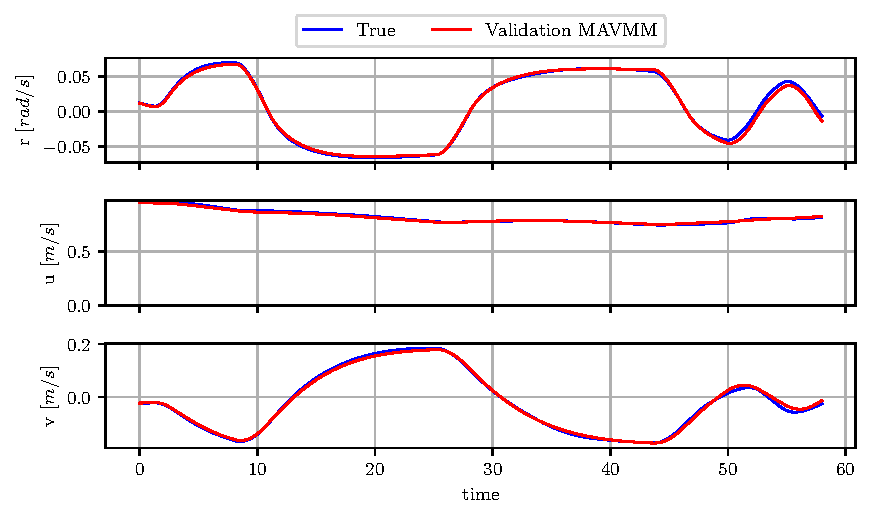
\includegraphics{kappa/images/9.pdf}
        \caption{Absolute correlation between the features in the wPCC yaw moment regression of AVMM}
        \label{fig:ncorr}
    \end{figure}
    
    \item The new method can predict turning circle manoeuvres with less than 5 \% error in advance and tactical diameter for the wPCC and KVLCC2 test cases. Track plot of the wPCC result is shown in Fig.\ref{fig:turning_circle_wpcc}.
    \begin{figure}[h]
    \centering
    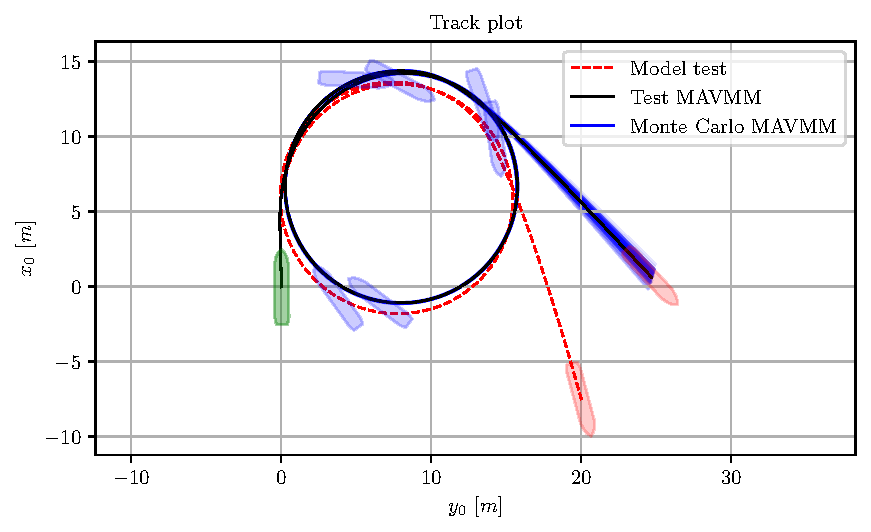
\includegraphics{kappa/images/10.pdf}
    \caption{Track plots of the turning circle test case for wPCC from Model test and simulation (Test). Also simulations with alternative realizations of the regression (Monte Carlo) are shown in this figure.}
    \label{fig:turning_circle_wpcc}
    \end{figure}
    
\end{itemize}







%%%%%%%%%%%%%%%%%%%%%%%%%%%%%%%
%%%%%%%%%%%%%%%%%%%%%%%%%%%%%%%
\chapter{Conclusions\label{ch:conclusions}}
%%%%%%%%%%%%%%%%%%%%%%%%%%%%%%%
The main conclusions are presented below with respect to the main objective of this thesis:
% Objective: 
\begin{quote} 
\expandafter\MakeUppercase \objective
\end{quote}
\noindent The conclusions are categorized by the identified goals to achieve this objective.

\subsubsection*{Roll model}
The first goal of the thesis was to develop a model for the calm water ship rigid body dynamics in the roll degree of freedom, based on model test data. 
Three candidate models were considered: 
\begin{itemize}
    \item the linear roll motion model
    \item the quadratic roll motion model
    \item the cubic roll motion model
\end{itemize}
\noindent Data from 250 roll decay tests obtained from SSPA were used to evaluate these models. The accuracy of the linear model was not as good as the nonlinear models. The quadratic model had almost as high accuracy as the cubic model and is expected to have better generalization with fewer parameter in the model. The quadratic model, is therefore the best choice to describe the roll motion. 

Predictions with original Ikeda's method was also conducted for some of the ships that exceeded the limits of the simplified Ikeda's method. These predictions were in much better agreement with the dampings from the model tests. This shows that the observed deviations with the simplified Ikeda's method are result from extrapolation errors rather than inherent 
errors in the original Ikeda's method.

A grey-box correction model of the simplified Ikeda's method and a complete black-box model to predict ship roll damping was proposed in Paper \ref{pap:rolldamping}. The proposed models give better predictions than the simplified Ikeda's method outside its limits but worse predictions within it. Applying corrections to the simplified Ikeda's method outside its limits is therefore not enough to get good roll damping predictions for modern ships. Further
research efforts should be devoted to creating an updated version of the simplified Ikeda's method.

\subsubsection*{Manoeuvring model}
The second goal in this thesis was to increase the complexity and uncertainty of the modelling by adding the surge, sway and yaw degrees of freedoms, addressing the manoeuvring problem.

It is shown in Paper \ref{pap:pit} that the hydrodynamic derivatives within a manoeuvring model can be identified exactly at ideal conditions with no measurement noise and a perfect estimator. 
This type of result can be seen when identifying parameters in a manoeuvring model on data from simulations with the same manoeuvring model.
The challenge in system identification on actual model test data is therefore to handle the measurement noise and the model uncertainty. A new system identification method has therefore been proposed in Paper \ref{pap:pit} where a preprocessor with EKF and RTS smoother are run in iteration for a set of candidate manoeuvring models to both handle the measurement noise and model uncertainty.
The system identification with the proposed preprocessor has higher accuracy than if low-pass filters are used and avoids the problem of finding the optimal cut-off frequency.

The linearization in the EKF may cause stability problems. This can be a problem for sparse time series, with longer time steps. This was however not a problem for the present test cases, with very high frequency data (100 Hz). 
Using unscented Kalman filter (UKF) instead of EKF is a possible solution, if these kinds of stability problems occur. This has however not been further investigated in this thesis.

Multicollinearity was a significant problem with the AVMM for both the wPCC and KVLCC2 data. Consequently, some of the regressed hydrodynamic derivatives in the AVMM have unphysically large values and substantial uncertainties. The model is still mathematically correct, where the regressed polynomials fit the training data well. The regressed polynomial could be the sum of large counteracting coefficients. The model works as long as the states are similar to the training data. However, when extrapolating, it is easy to imagine that the balance between these massive derivatives is disturbed, giving significant extrapolation errors very quickly. This behavior was seen when predicting forces and moments with the AVMM on unseen validation data and is a well known problem \cite{ittc_maneuvering_2008}.
The MAVMM has fewer hydrodynamic derivatives with lower multicollinearity and minor extrapolation errors. Including propeller thrust in the manoeuvring model made it possible to obtain high accuracy with fewer hydrodynamic derivatives. Another problem with a too many parameters in a model is that the standard manoeuvres used in this paper does not follow the aspect of persistence of excitation, so that some of the hydrodynamic derivatives might not be identifiable \cite{revestido_herrero_two-step_2012}. During zigzag tests, the model is for instance exposed to only two rudder angles for a majority of the data. A series of step responses as used in \cite{miller_ship_2021} gives a better excitation, but requires a lot of space, which is possible at lake experiments, but not in a narrow basin. The model generalization therefore needs to be addressed, as seen in the next section.

\subsubsection*{Model generalization} 
The third goal of this thesis was model generalization. The models must be able to make predictions outside the domain covered by the available data, in order to be of practical use in Internet of Ships (IoS) applications. A model development process for manoeuvring models with good generalization was proposed in Paper \ref{pap:pit}.
The process was applied together with the proposed parameter estimation technique on the wPCC and KVLCC2 test cases. Turning circles where predicted with good accuracy on models trained on zigzag tests. This shows that the models have good generalization, since the turning circles have much larger rudder angles, drift angles and yaw rates, compared to the training zigzag tests. 

%%%%%%%%%%%%%%%%%%%%%%%%%%%%%%%
%%%%%%%%%%%%%%%%%%%%%%%%%%%%%%%
\chapter{Future work\label{ch:future_work}}
%%%%%%%%%%%%%%%%%%%%%%%%%%%%%%%

\subsubsection*{New generic roll damping model}
The PIT of the roll motion models applied on 250 roll-decay tests that was investigated in Paper \ref{pap:rolldamping} produced a roll damping database for modern ship types. A grey-box model and a black-box model as described in Section \ref{sec:genericrolldampingmodel} was developed from this database. The prediction accuracy of these models were not very good and should be improved. This is important, especially since the SI method, being the state of art white-box physical model for roll damping, was found to be outside its limits for the ships in the database. This implies that there is a need for a new roll damping prediction method for modern ships.  

\subsubsection*{Black-box model}
Investigate black-box models, as an alternative to the grey-box models proposed in this thesis and compare with respect to accuracy and generalization.

\subsubsection*{Model for sailing digital twin}
Develop models from wPCC sailing model tests for the future sailing ship digital twins.

\subsubsection*{Manoeuvring system identification on 100 ships}
Expanding the analysis of the two ships from Paper \ref{pap:pit} to 100 ships tested at SSPA Sweden AB.

\subsubsection*{System identification of ship rigid body dynamics in wind and waves}

\subsubsection*{System identification of ship rigid body dynamics in full scale calm waters}

  

\printbibliography[heading=bibintoc]

%  \end{refsection}

\cleardoublepage

%\printbibliography[heading=subbibintoc] % biblatex bibliography


% % % Preparations before Part II. In this part one chapter = one paper

\renewcommand{\chaptername}{Paper}
                              % write 'Paper' instead of 'Chapter' in the title

\setcounter{chapter}{0}       % reset chapter numbers after Part I

% Fix hyperlinks to chapters/papers after chapter counter reset, see
% http://tex.stackexchange.com/a/6099
\renewcommand\theHchapter{appendedPaper.\arabic{chapter}}

\renewcommand{\thesection}{\arabic{section}}
                              % exclude chapter number from section number
                              % Figures, Tables, etc are still prefixed by chapter number.
                              % For algorithms numbering see definition of
                              % \newfloat{algorithm} above.

\newcommand{\paper}[7]
% #1 Paper Title
% #2 Short Title for page headers (ToC has the full title)
% #3 Label for later (or earlier) \ref:s
% #4 Authors
% #5 Where published
% #6 Comment (like "reprinted with a kind permission" and "reformatted for uniformity")
% #7 File to input
{
  \chapter{#1\label{#3}}      % Title as Chapter
  \chaptermark{#2}            % Short title for the page header
  \thispagestyle{empty}       % no page numbers
  {\Large #4}\par             % authors
  \vspace{1cm}
  \noindent\emph{\Large #5}\par % where published
  \vspace{3cm}
  \noindent\emph{\Large #6}   % Comment
%  \cleardoublepage            % skip back side of the page
%  \thispagestyle{plain}       % no header above paper title
%  \begin{center}
%    {\Large \bfseries Paper~\thechapter. #1}\par % title again
%    \vspace{1pc}
%    #4 \par                   % authors again
%    \vspace{3pc}
%  \end{center}
%  \begin{refsection}          % start of biblatex's refsection for sub-bibliography
%  \input{#7}                  % paper itself, starting from abstract (no title)
%  \printbibliography[heading=subbibintoc] % biblatex bibliography
%  \end{refsection}            % end of biblatex refsection
}

\newcommand{\reformatted}{The paper was reformatted for uniformity, but otherwise is unchanged.}

\addtocontents{toc}{\cftpagenumbersoff{chapter}}

\part{Appended papers}        % in this part one chapter = one paper

% Example of using the command \paper defined above: 
\paper{Analysis of roll damping model scale data}
      {~}
      {pap:rolldamping}
      {Martin Alexandersson, Wengang Mao and Jonas Ringsberg}
      {Ships and Offshore Structures 16.sup1. Publisher: Taylor \& Francis}
      {~}

\paper{A comparison of ship manoeuvrability models to approximate ship navigation trajectories}
      {~}
      {pap:daiyong}
      {Martin Alexandersson, Daiyong Zhang, Wengang Mao and Jonas Ringsberg}
      {Ships and Offshore Structures}
      {~}

\paper{System identification of {Vessel} {Manoeuvring} {Models}}
      {~}
      {pap:pit}
      {Martin Alexandersson, Wengang Mao and Jonas Ringsberg}
      {Ocean Engineering}
      {~}

\end{document}
